\documentclass[compress]{beamer}
\usefonttheme{professionalfonts}



%

\usepackage[T1]{fontenc}
%\usepackage{kmath,kerkis}
%\usepackage{fouriernc}
\usepackage[adobe-utopia]{mathdesign}
%\usepackage{arev}
\usepackage{times}
\usepackage{natbib}

\usepackage[noend]{algpseudocode}
\usepackage{xmpmulti}
\usepackage{dsfont}
\usepackage{amsmath}

\usepackage{graphicx,float,wrapfig, bbm}
\usepackage{amsfonts, comment, bbold}
\usepackage{mdwlist}
\usepackage{subfigure}
\usepackage{colortbl}
\usepackage{mathrsfs}


\usepackage{multirow}




% packages

\usepackage{amsfonts}

% environments

\newenvironment{packed_enumerate}{
  \begin{enumerate}
    \setlength{\topsep}{0pt}
    \setlength{\itemsep}{2pt}
    \setlength{\parskip}{0pt}
    \setlength{\parsep}{0pt}
}{\end{enumerate}}

\newenvironment{stepit}
 {\begin{itemize}[<+-|alert@+>]}
   {\end{itemize}}

% commands

\newcommand{\Norm}[3]{\mathcal{N}\left( #1, #2, #3 \right)}
\newcommand{\popshow}[2]{\only<#1->{\alert<#1>{#2}}}
\newcommand{\x}{\mathbf{x}}
\newcommand{\ex}[1]{\mbox{exp}\left\{ #1\right\} }
\newcommand{\e}[2]{\mathbb{E}_{#1}\left[ #2 \right] }
\newcommand{\g}{\, | \,}
\newcommand{\indpt}{\protect\mathpalette{\protect\independenT}{\perp}}
\def\independenT#1#2{\mathrel{\rlap{$#1#2$}\mkern2mu{#1#2}}}
\newcommand{\E}{\textrm{E}}
\newcommand{\R}{\textrm{R}}
\newcommand{\realline}{\mathbb{R}}
\newcommand{\data}{{\cal D}}
\newcommand{\loglik}{{\cal L}}
\newcommand{\grad}[2]{ \frac{\partial{#1}}{\partial#2}}
\newcommand{\dir}[1]{\mbox{Dir}(#1)}
\newcommand{\mult}[1]{\mbox{Mult}( #1)}
\newcommand{\G}[1]{\Gamma \left( \textstyle #1 \right)}
\newcommand{\ind}[1]{\mathds{1}\left[ #1 \right] }
\newcommand{\norm}[1]{\left\lVert#1\right\rVert}

\newcommand{\class}[1]{ \texttt{#1}}
\newcommand{\term}[1]{ ``#1''}
\newcommand{\tcword}[0]{ w }
\newcommand{\docsetlabeled}[0]{ D }
\newcommand{\onedoclabeled}[0]{ d }
\newcommand{\tcposindex}[0]{ i }
\newcommand{\myblue}[1]{ {\textbf #1 }}
\newcommand{\dnrm}[1]{ _{\mbox{\textsc{ #1 }}}}
\newcommand{\argmax}[0]{ \arg \max }
\newcommand{\tcjclass}[0]{c_j}
\newcommand{\maths}[1]{ {\bf #1}}




% complexity
\renewcommand{\O}{\mathcal{O}}



\setbeamersize{text margin left=0.5cm}
\setbeamersize{text margin right=0.5cm}
\setbeamercolor{alert}{fg=red!75!black}

\usetheme{default}
\useinnertheme{circles}
\useoutertheme{split}
\usecolortheme{seahorse}
% \usecolortheme{dove}
% \usecolortheme{seagull}
%\usecolortheme{default}
% \usecolortheme{dolphin}
\usefonttheme{structurebold}
%\usefonttheme{serif}

\setbeamertemplate{navigation symbols}{}
\setbeamertemplate{headline}{}
\setbeamertemplate{footline}{}
\setbeamerfont{itemize/enumerate subbody}{size=\normalsize}
\setbeamerfont{itemize/enumerate subsubbody}{size=\normalsize}
\setbeamercolor{itemize item}{fg=gray}
\setbeamercolor{enumerate item}{fg=gray}
\setbeamercolor{itemize item}{fg=gray}
\setbeamercolor{itemize subitem}{fg=gray}
\setbeamercolor{item projected}{bg=gray}
\setbeamercolor{subitem projected}{bg=gray}


\newenvironment{bullets}
{\begin{itemize} \setlength{\itemsep}{10pt}}
{\end{itemize}}

\newcommand{\mygraphic}[2]{
  \begin{beamercolorbox}[colorsep*=4pt]{black math}
    \begin{center}
      \includegraphics[#1]{#2}
    \end{center}
  \end{beamercolorbox}
}

\setbeamercolor{structure}{bg=gray}
\setbeamercolor{section in head/foot}{bg=gray}
\setbeamercolor{palette primary}{bg=lightgray}


\usepackage{minted}

\usetheme[pageofpages=of,                    % String used between the current page and the
                                             % total page count.
          bullet=circle,                     % Use circles instead of squares for bullets.
          titleline=true,                    % Show a line below the frame title.
          showdate=true,                     % show the date on the title page
          alternativetitlepage=true,         % Use the fancy title page.
          titlepagelogo=../../common/culogo,              % Logo for the first page.
          % Logo for the header on first page.
          headerlogo=../../common/boulder_cs,
          ]{UCBoulder}

\usecolortheme{ucdblack}
\author{Introduction to Data Science Algorithms}


\institute[Boyd-Graber and Paul] % (optional, but mostly needed)
{Jordan Boyd-Graber and Michael Paul}


\AtBeginSection[] % "Beamer, do the following at the start of every section"
{ \begin{frame} \frametitle{Outline} % make a frame titled "Outline"
\tableofcontents[currentsection] % show TOC and highlight current section
\end{frame} }


\usepackage{amsmath}
\usepackage{bm}

\newcommand{\gfx}[2]{
\begin{center}
	\includegraphics[width=#2\linewidth]{topic_models/#1}
\end{center}
}
\title{Topic Models}
\date{Overview}

\begin{document}


\frame{\titlepage
}

\begin{frame}{Learning the Hidden Space}

  \begin{itemize}
    \item Two major tools:
      \begin{itemize}
        \item Gibbs Sampling: Easier to implement, easier to understand
        \item Variational Inference: faster, harder to implement
      \end{itemize}
    \item Variational shows the connections to ``deep'' models better, so it's the focus
    \item However, would be injustice to not at least discuss Gibbs sampling
  \end{itemize}

\end{frame}

%

\providecommand{\graphscale}{0.6}




\begin{frame}

	\frametitle{Why topic models?}

	\begin{columns}

	\column{.3\linewidth}

	
\includegraphics[width=1\linewidth]{topic_models/newspapers}

	\column{.55\linewidth}

	\begin{itemize}
		\item Suppose you have a huge number of documents
		\item Want to know what's going on
		\item Can't read them all (e.g. every New York Times article from the 90's)
		\item Topic models offer a way to get a corpus-level view of major themes
		\pause
		\item Unsupervised
	\end{itemize}


	\end{columns}

\end{frame}

\begin{frame}{Roadmap}

	\begin{itemize}
		\item What are topic models
		\item How to know if you have good topic model
		\item How to go from raw data to topics
	\end{itemize}

\end{frame}


\frame{
\begin{center}
\frametitle{Embedding Space}
From an \textbf<1>{input corpus} and number of topics \textbf<1>{$K$} $\rightarrow$ \textbf<2>{words to topics} \\
\only<1>{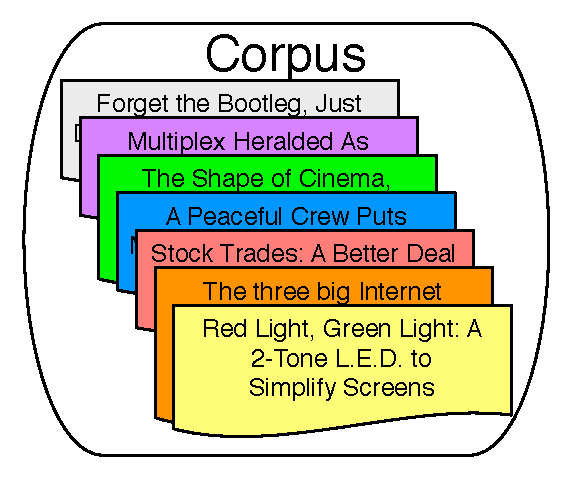
\includegraphics[width=0.6\linewidth]{topic_models/reading_tea_leaves/heldout_0} }
\only<2>{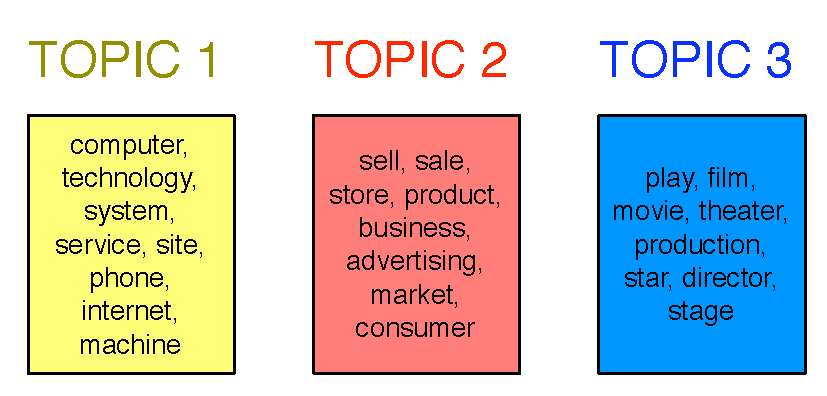
\includegraphics[width=0.9\linewidth]{topic_models/reading_tea_leaves/nyt_topics_wide}}
\end{center}
}

\frame{\frametitle{Conceptual Approach}

\begin{itemize}
\item For each document, what topics are expressed by that document?

\begin{center}
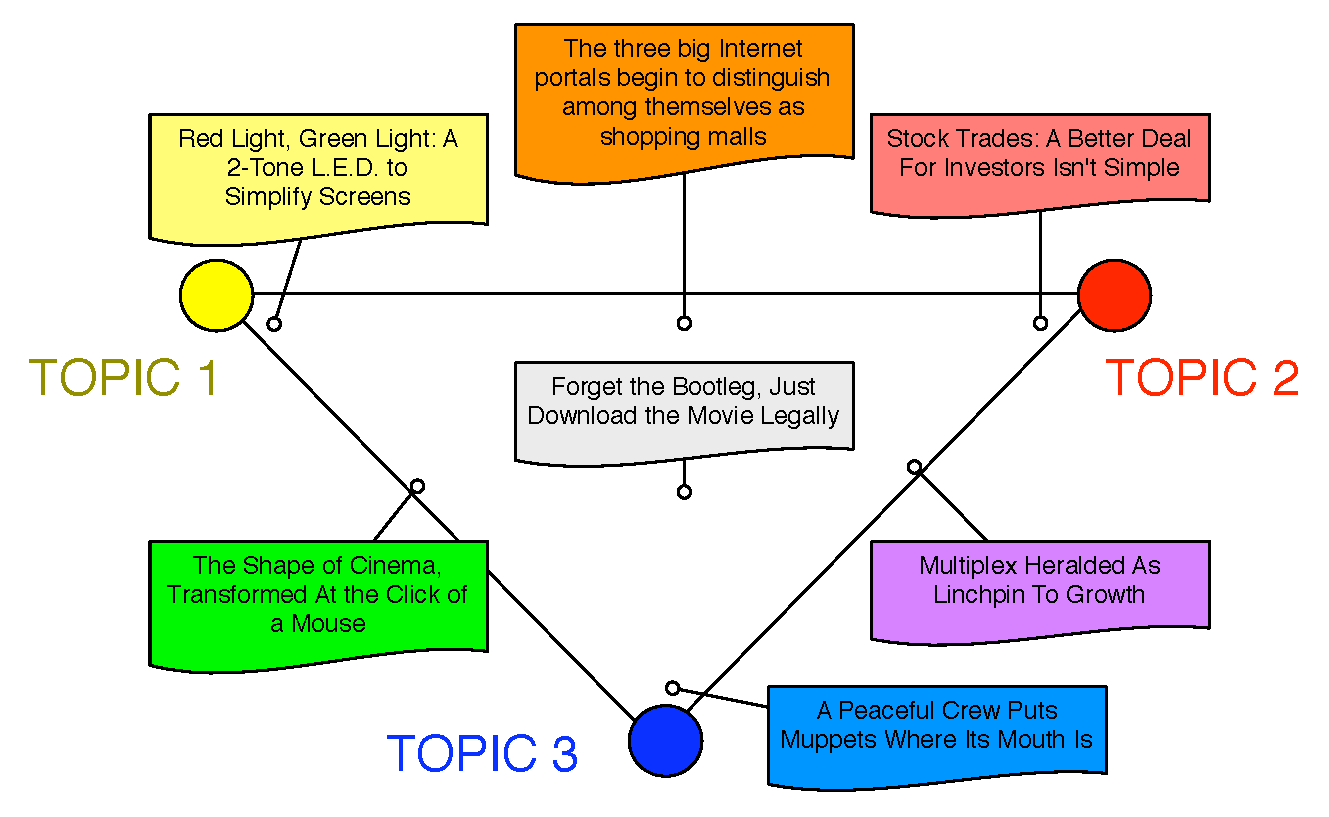
\includegraphics[width=0.9\linewidth]{topic_models/nyt_documents}
\end{center}

\end{itemize}
}



\begin{frame}

\frametitle{Topics from \emph{Science}}

\begin{center}
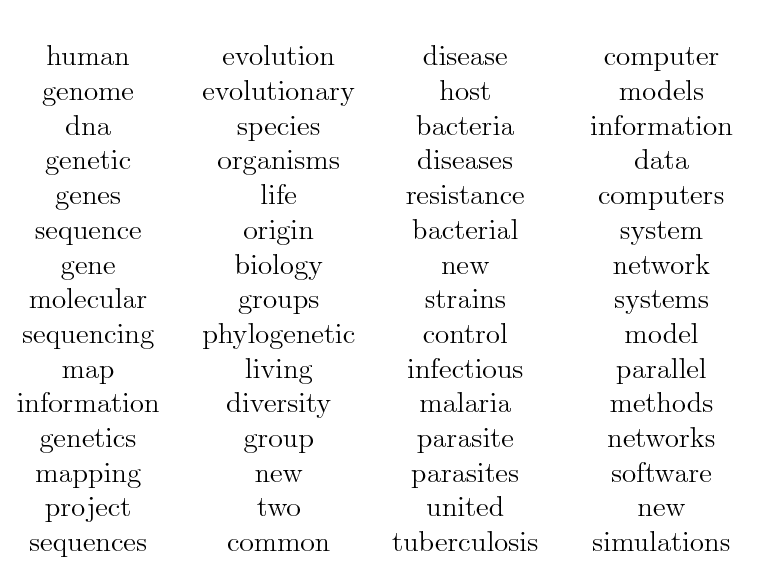
\includegraphics[width=0.8\linewidth]{topic_models/example_topics}
\end{center}

\end{frame}


\begin{frame}

\frametitle{Why should you care?}

\begin{itemize}
\item Neat way to explore / understand corpus collections
\begin{itemize}
	\item E-discovery
	\item Social media
	\item Scientific data
\end{itemize}
\item NLP Applications
\begin{itemize}
   \item Word Sense Disambiguation
   \item Discourse Segmentation
   \item Machine Translation
\end{itemize}
\item Psychology: word meaning, polysemy
\item Inference is (relatively) simple
\end{itemize}

\end{frame}

\frame
{
  \frametitle{Matrix Factorization Approach}

\begin{center}
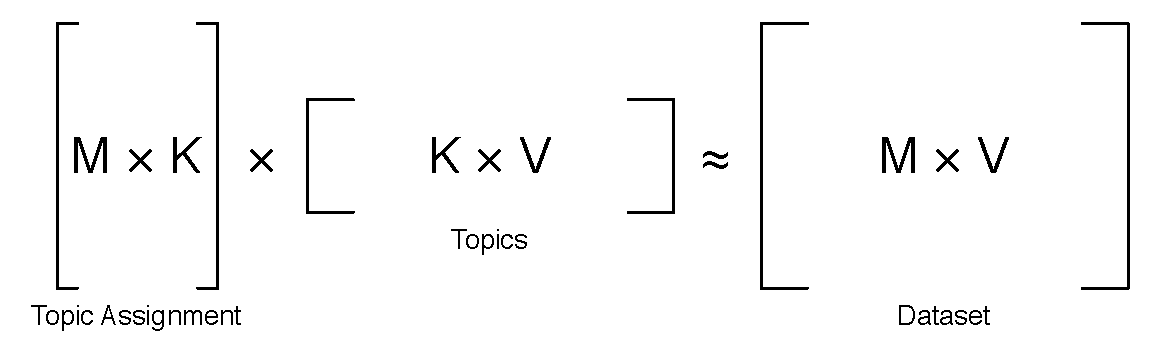
\includegraphics[width=0.9\linewidth]{topic_models/factorization.pdf}
\end{center}

\begin{columns}
\column{.5\textwidth}
\begin{block}{}
	\begin{itemize}
		\item[K] Number of topics
		\item[M] Number of documents
		\item[V] Size of vocabulary
	\end{itemize}
\end{block}
\column{.5\textwidth}
\pause
\begin{itemize}
\item If you use singular value decomposition (SVD), this technique is called latent semantic analysis.
\item Popular in information retrieval.
\end{itemize}
\end{columns}

}

\begin{frame}

\frametitle{Alternative: Generative Model}

\begin{itemize}
  \item How your data came to be
  \item Sequence of Probabilistic Steps
  \item Posterior Inference
    \pause
  \item Blei, Ng, Jordan.  Latent {\bf Dirichlet} Allocation.  JMLR, 2003.
\end{itemize}

\end{frame}

\begin{frame}
	\frametitle{Multinomial Distribution}

	\begin{itemize}
		\item Distribution over discrete outcomes
		\item Represented by non-negative vector that sums to one
		\item Picture representation
	\begin{center}
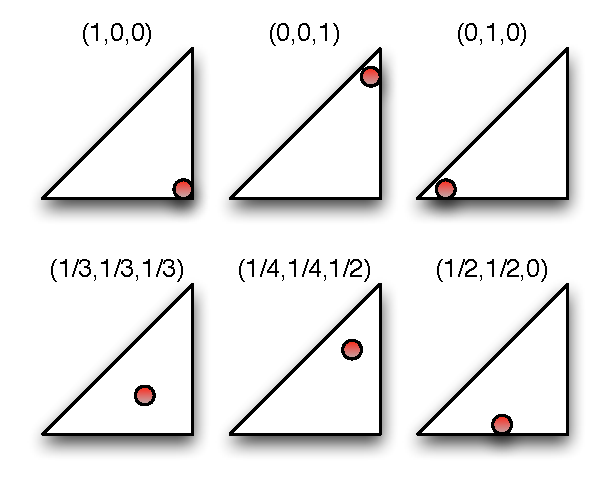
\includegraphics[width=0.4\linewidth]{topic_models/multinomial}
	\end{center}
		\pause
		\item Come from a Dirichlet distribution

	\end{itemize}


\end{frame}

\begin{frame}

\frametitle{Dirichlet Distribution}

\begin{center}
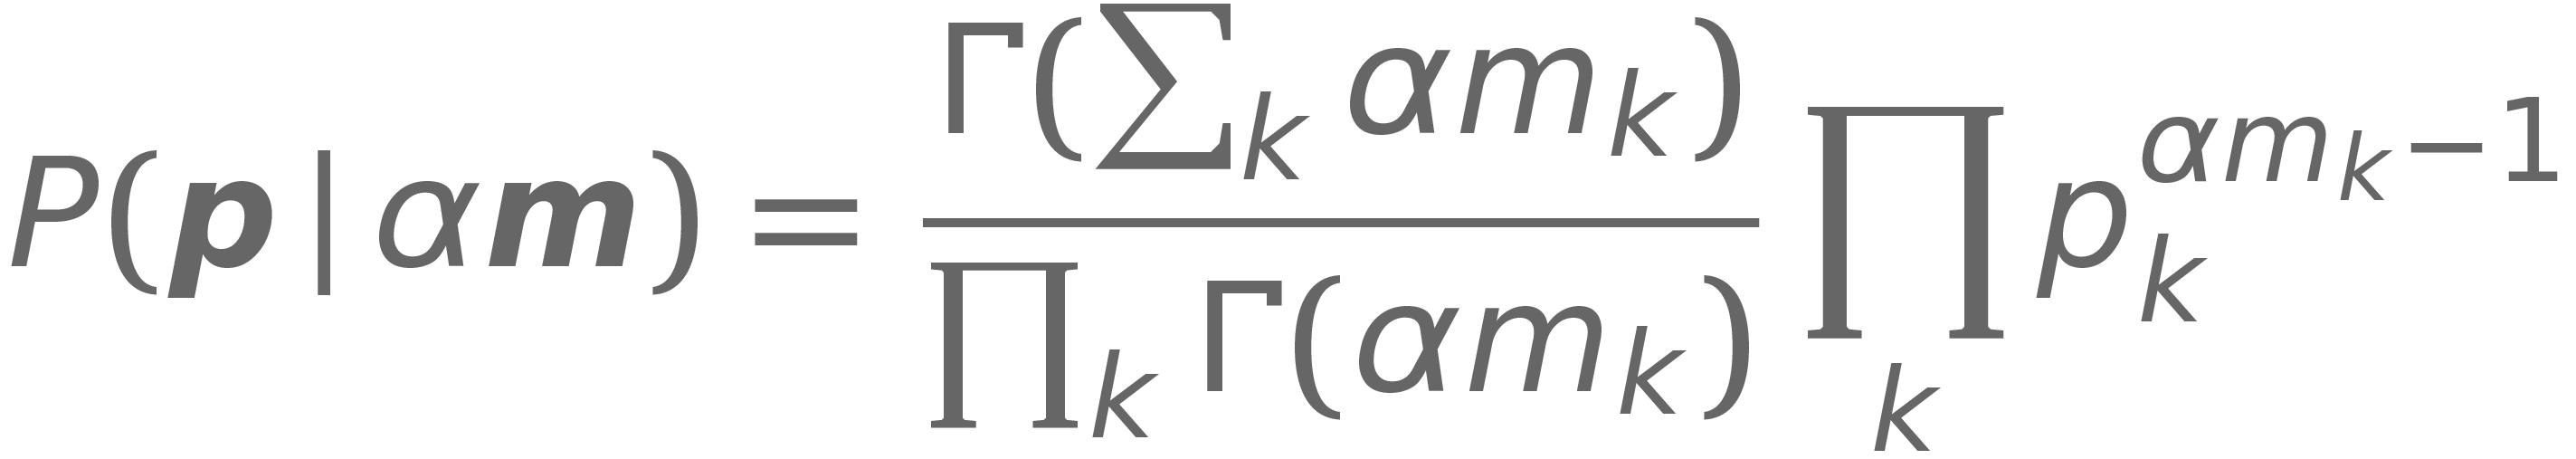
\includegraphics[width=0.4\linewidth]{topic_models/equations/dirichlet} \\ \bigskip
\pause
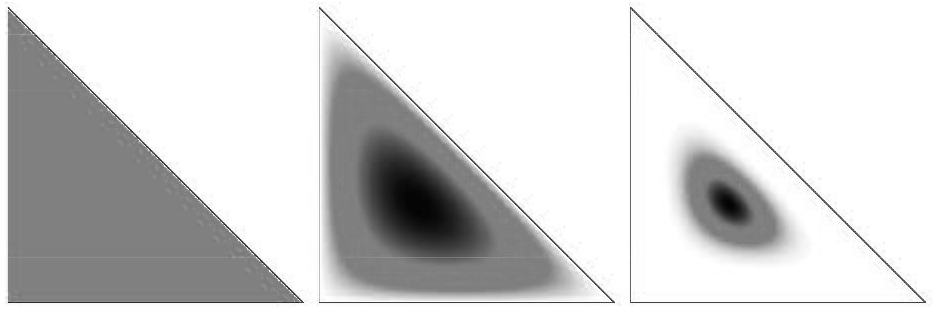
\includegraphics[width=0.6\linewidth]{topic_models/dirichlet_1} \\
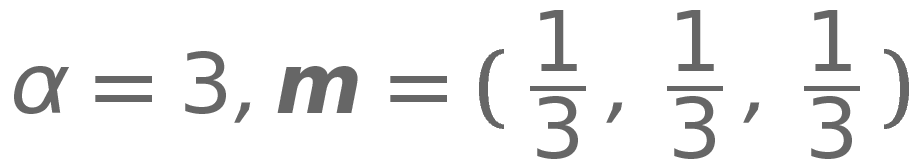
\includegraphics[width=0.2\linewidth]{topic_models/equations/dirichlet_params_1} 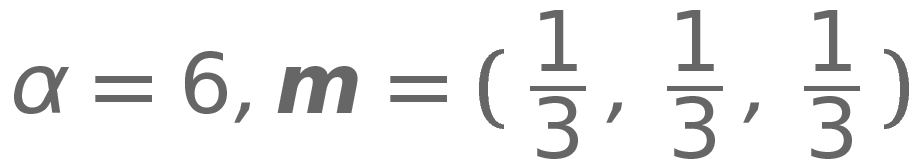
\includegraphics[width=0.2\linewidth]{topic_models/equations/dirichlet_params_2} 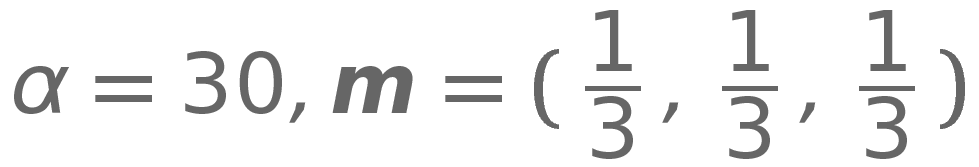
\includegraphics[width=0.2\linewidth]{topic_models/equations/dirichlet_params_3} \\
\pause
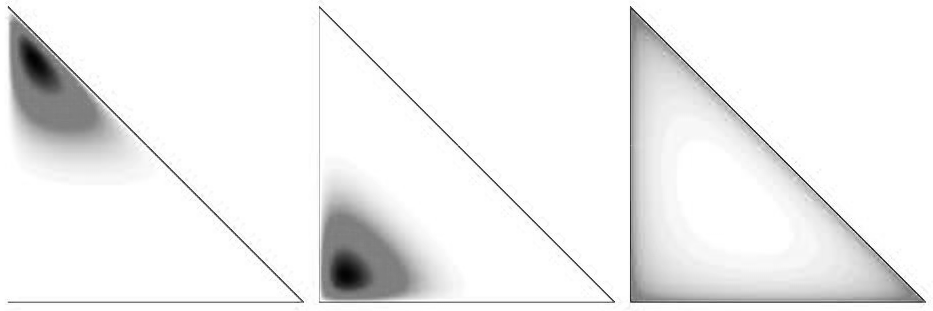
\includegraphics[width=0.6\linewidth]{topic_models/dirichlet_2} \\
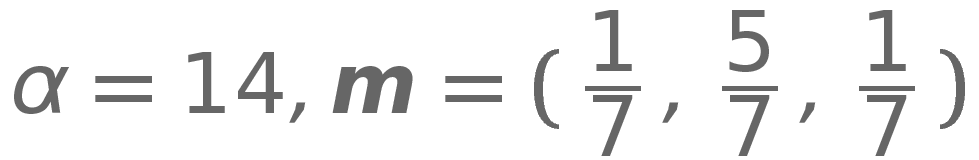
\includegraphics[width=0.2\linewidth]{topic_models/equations/dirichlet_params_4} 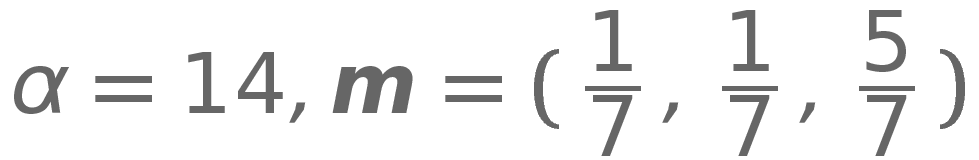
\includegraphics[width=0.2\linewidth]{topic_models/equations/dirichlet_params_5} 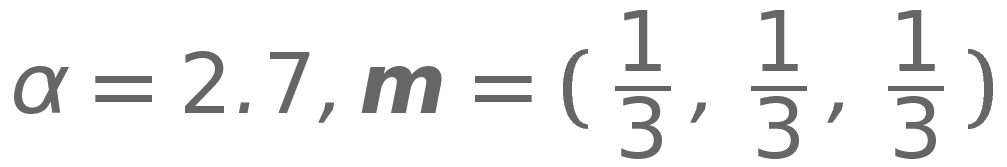
\includegraphics[width=0.2\linewidth]{topic_models/equations/dirichlet_params_6} \\
\end{center}

\end{frame}

\begin{frame}
\frametitle{Dirichlet Distribution}
\begin{center}
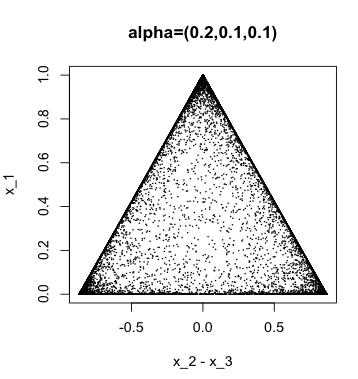
\includegraphics[width=0.5\linewidth]{topic_models/sparsity}
\end{center}
\end{frame}



\begin{frame}
\frametitle{Dirichlet Distribution}
\begin{itemize}
  \item If ${\bm \phi} \sim \dir(\alpha)$, ${\bm w} \sim \mult(\phi)$, and $n_k = |\{ w_i : w_i = k\}|$ then
  \begin{align}
  	p(\phi | \alpha, {\bm w}) & \propto p({\bm w} | \phi) p(\phi | \alpha) \\
	                       & \propto  \prod_{k} \phi^{n_k} \pause  \prod_k { \phi^{\alpha_k - 1}} \\
	                       & \propto \prod_k \phi^{\alpha_k + n_k - 1}
  \end{align}
  \item Conjugacy: this {\bf posterior} has the same form as the {\bf prior}
\end{itemize}
\end{frame}




\begin{frame}{Generative Model}
	\only<1> {   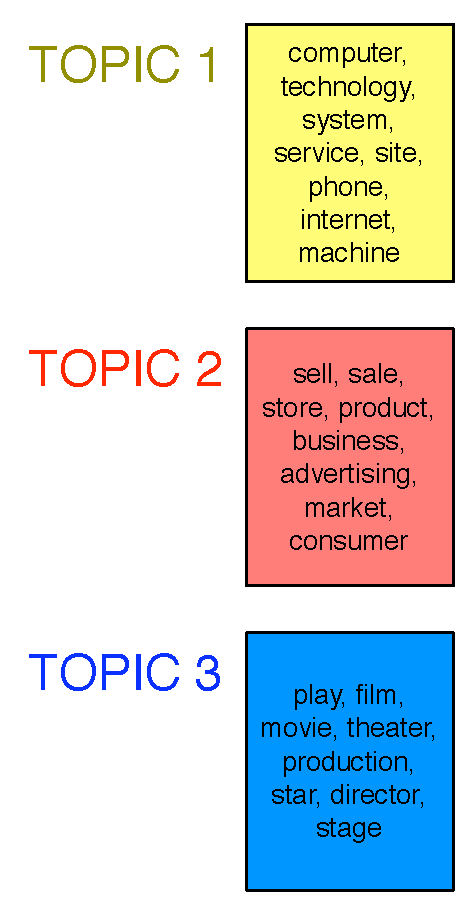
\includegraphics[width=.3\linewidth]{topic_models/nyt_topics}  }
	\only<2> {   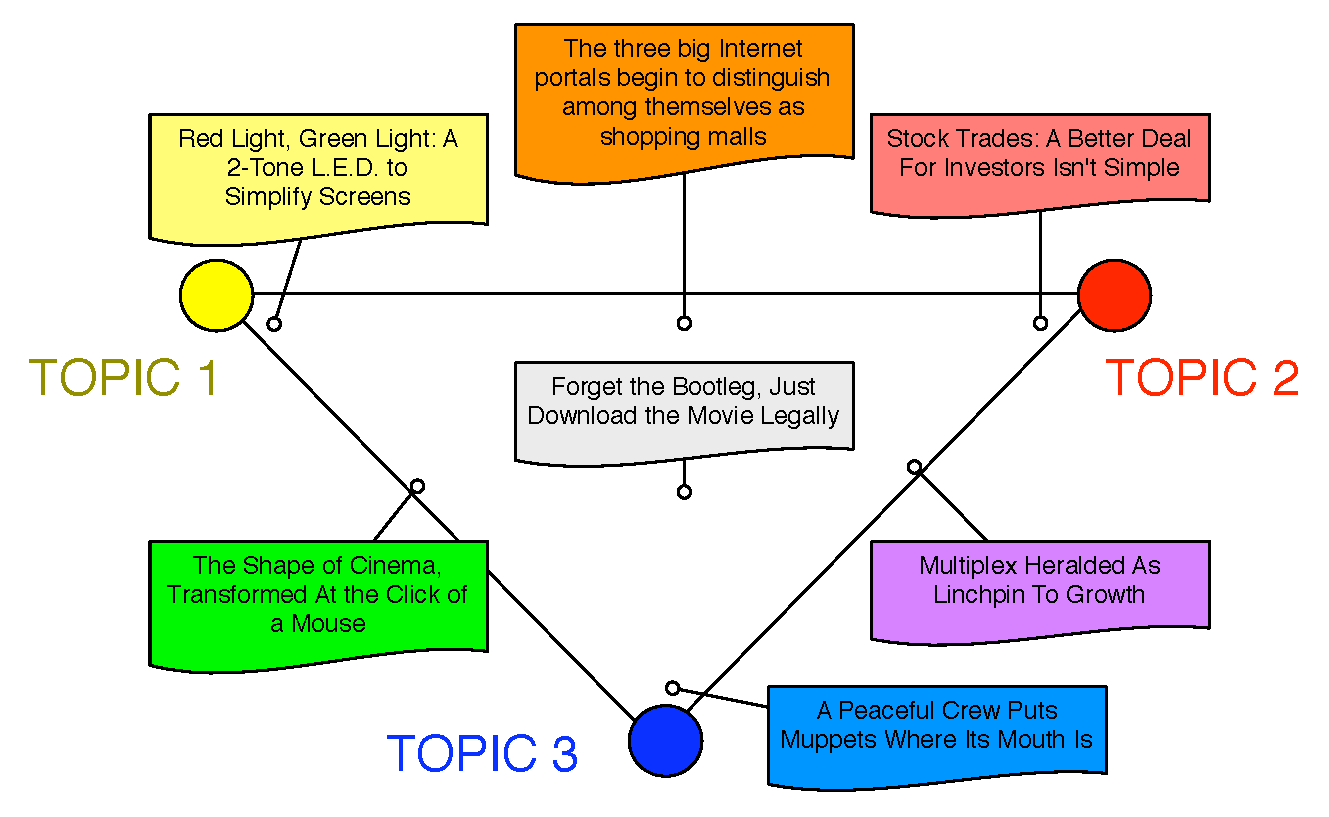
\includegraphics[width=.8\linewidth]{topic_models/nyt_documents}  }
	\only<3> {   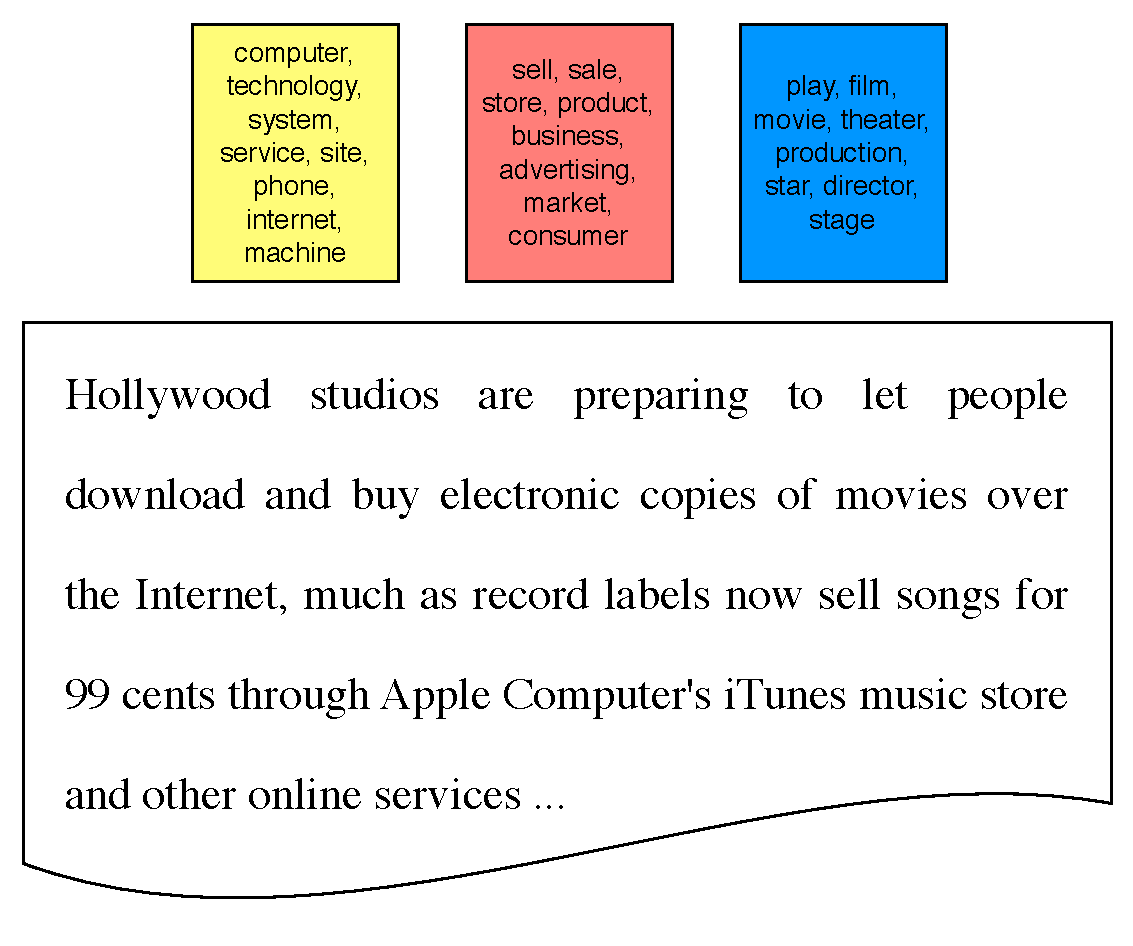
\includegraphics[width=.8\linewidth]{topic_models/inference_0}  }
	\only<4> {   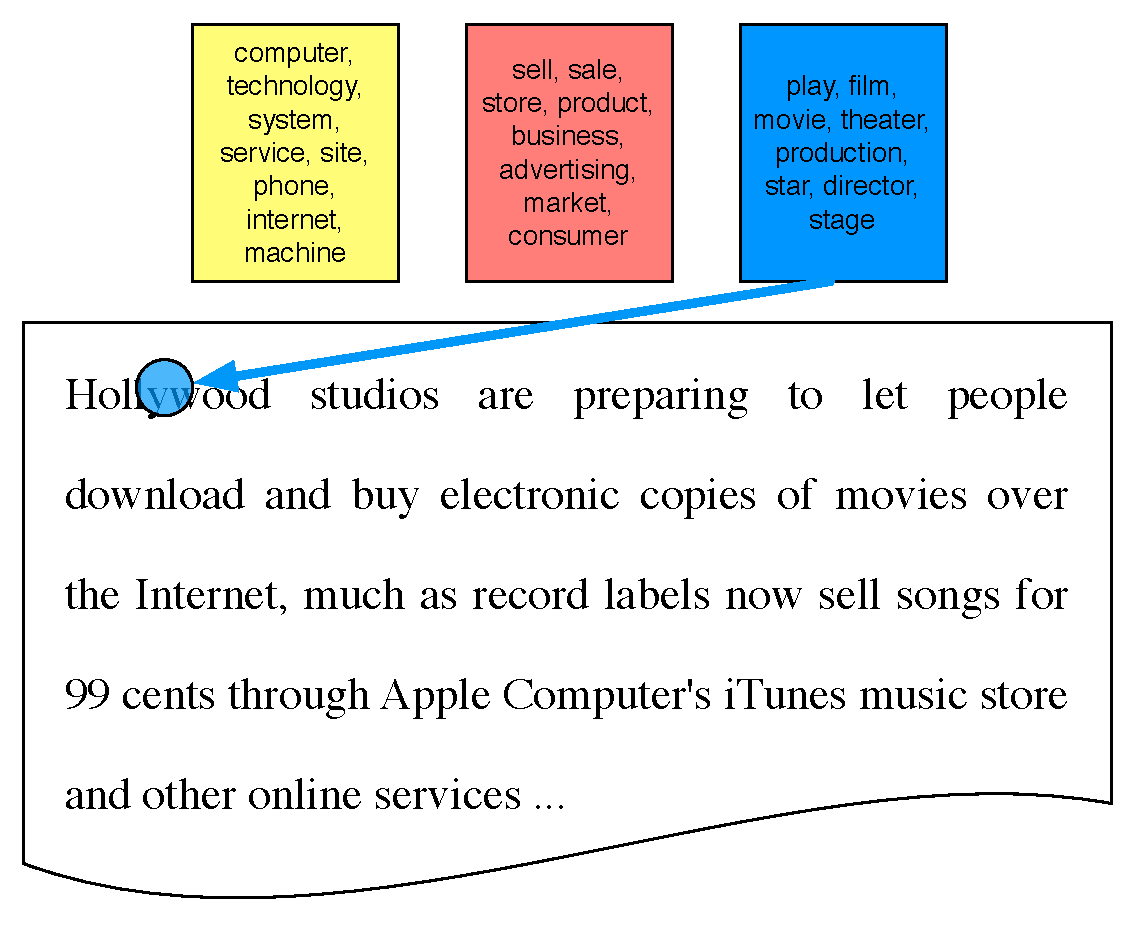
\includegraphics[width=.8\linewidth]{topic_models/inference_1}  }
	\only<5> {   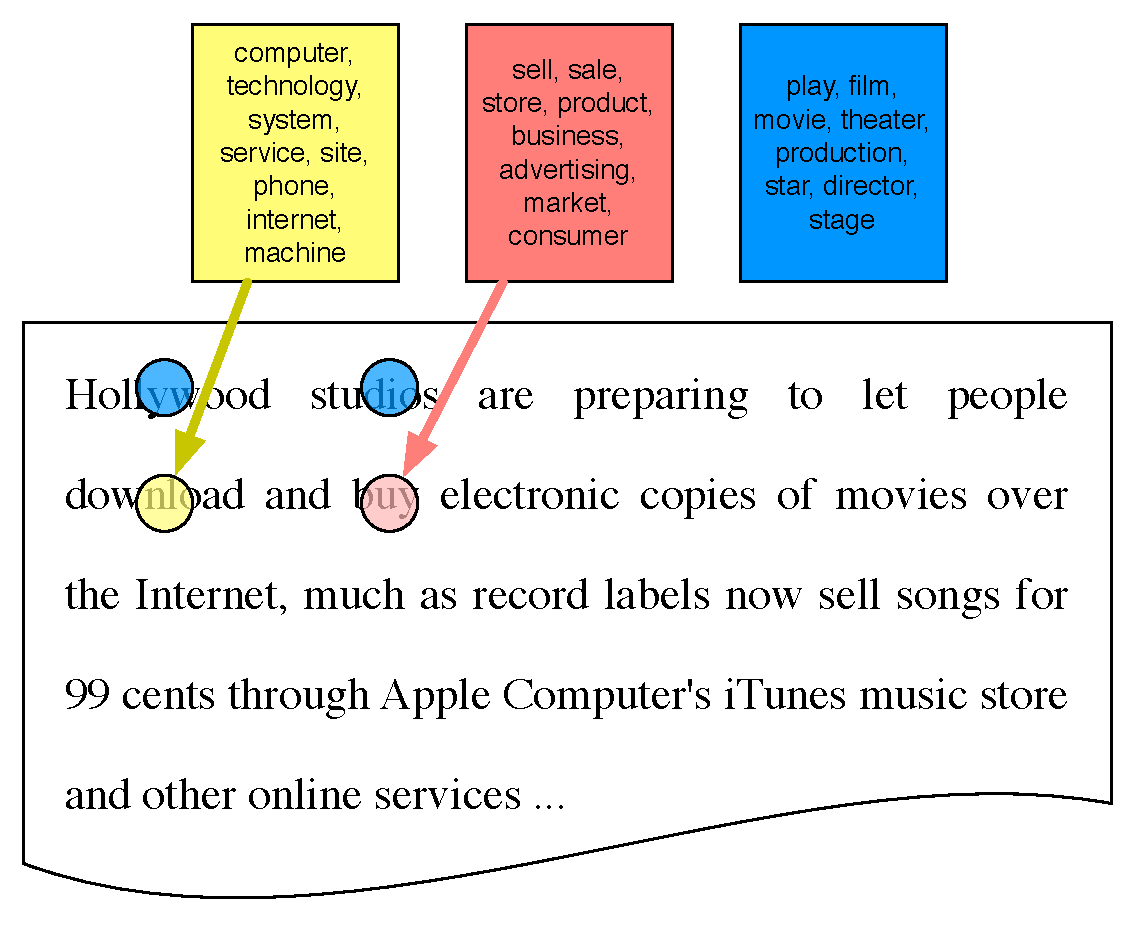
\includegraphics[width=.8\linewidth]{topic_models/inference_2}  }
	\only<6> {   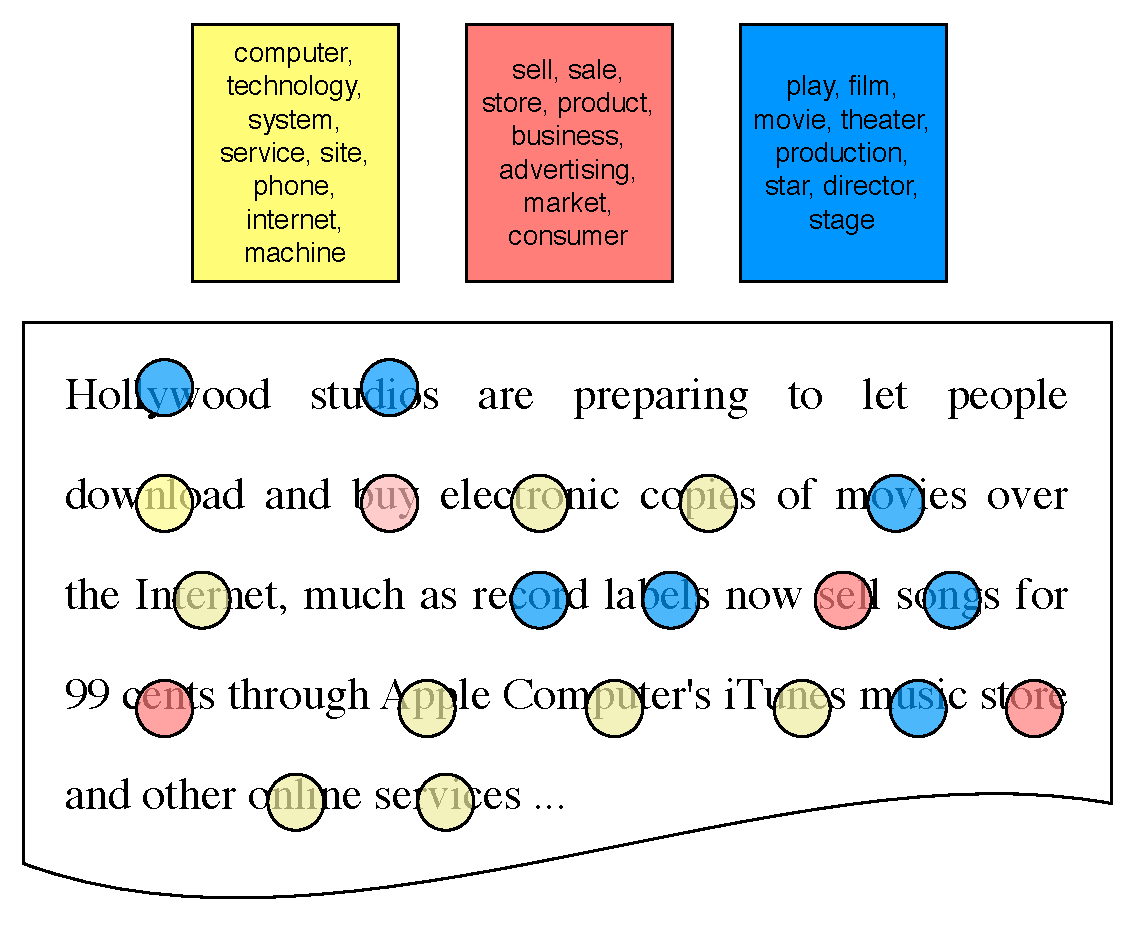
\includegraphics[width=.8\linewidth]{topic_models/inference_3}  }
\end{frame}

\frame
{
  \frametitle{Generative Model Approach}

\begin{center}
\only<1>{ 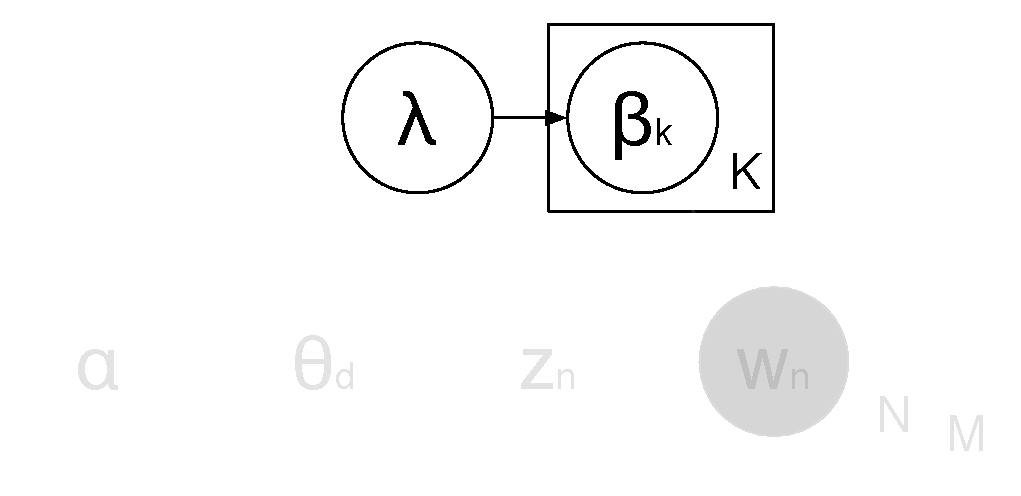
\includegraphics[scale=0.4]{topic_models/lda1.pdf} }
\only<2>{ 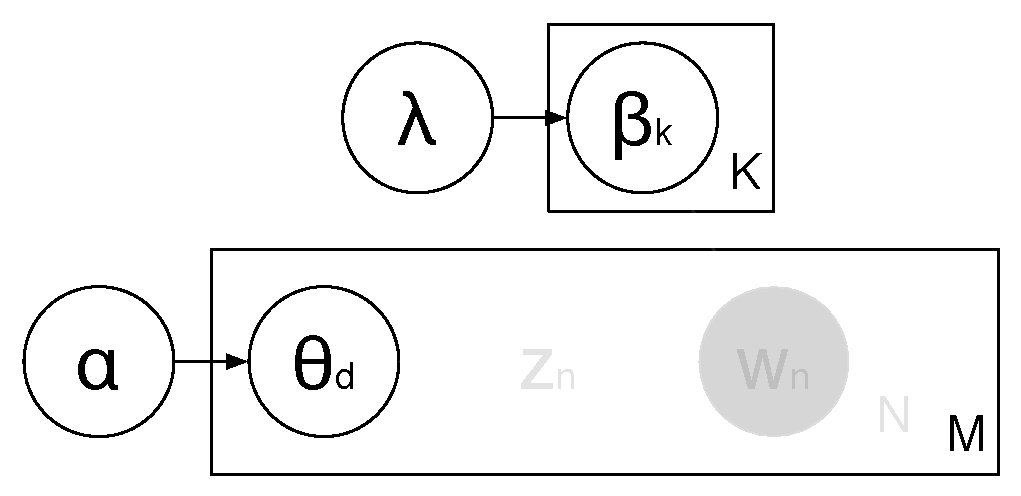
\includegraphics[scale=0.4]{topic_models/lda2.pdf} }
\only<3>{ 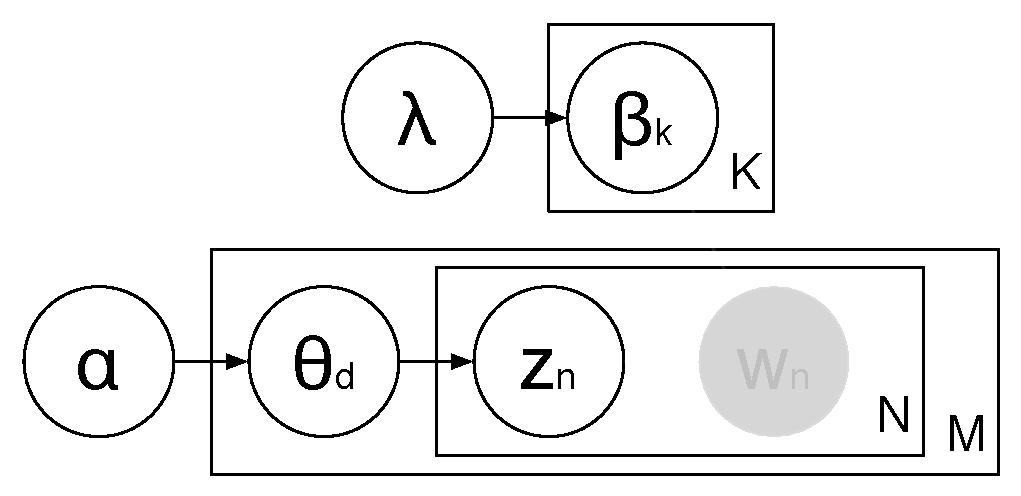
\includegraphics[scale=0.4]{topic_models/lda3.pdf} }
\only<4->{ 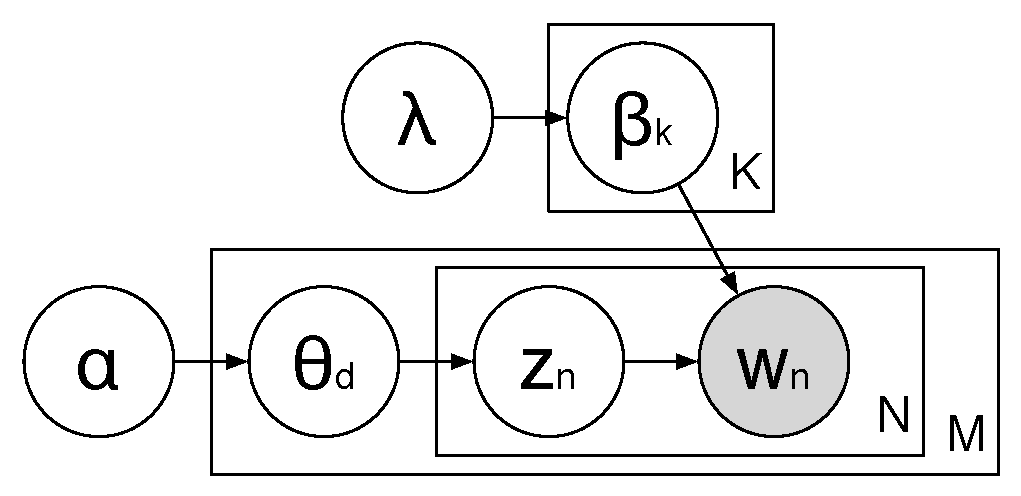
\includegraphics[scale=0.4]{topic_models/lda4.pdf} }
\end{center}

\begin{itemize}
\item<1-> For each topic $k \in \{1, \dots, K\}$, draw a multinomial distribution $\beta_k$ from a Dirichlet distribution with parameter $\lambda$
\item<2-> For each document $d \in \{1, \dots, M\}$, draw a multinomial distribution $\theta_d$ from a Dirichlet distribution with parameter $\alpha$
\item<3-> For each word position $n \in \{1, \dots, N\}$, select a hidden topic $z_n$ from the multinomial distribution parameterized by $\theta$.
\item<4-> Choose the observed word $w_n$ from the distribution $\beta_{z_n}$.
\end{itemize}

\only<5->{We use statistical inference to uncover the most likely unobserved variables given observed data.}
}

\begin{frame}
\frametitle{Topic Models: What's Important}
\begin{itemize}
\item Topic models \only<2>{(latent variables)}
\begin{itemize}
	\item Topics to word types---multinomial distribution
	\item Documents to topics---multinomial distribution
\end{itemize}
\item Focus in this talk: statistical methods
  \begin{itemize}
    \item Model: story of how your data came to be
    \item Latent variables: missing pieces of your story
    \item Statistical inference: filling in those missing pieces
  \end{itemize}
\item We use latent Dirichlet allocation (LDA), a fully Bayesian
  version of pLSI, probabilistic version of
  LSA
\end{itemize}

\end{frame}


\providecommand{\dirfunc}[3]{ \frac{ \prod_{#1}^{#2} \G{ #3 }} { \G{ \sum_{#1}^{#2} #3 }}}
\providecommand{\dirnum}[4]{ \frac{\G{ #3 }}{#4} \prod_{#1}^{#2} }
\providecommand{\dirden}[3]{ \G{ \sum_{#1}^{#2} #3 } }


\begin{frame}
\frametitle{Inference}

\begin{itemize}
\item We are interested in posterior distribution
\begin{equation}
p(Z | X, \Theta)
\end{equation}
\pause
\item Here, latent variables are topic assignments $z$ and topics $\theta$.  $X$ is the words (divided into documents), and $\Theta$ are hyperparameters to Dirichlet distributions: $\alpha$ for topic proportion, $\lambda$ for topics.
\begin{equation}
p({\bm z}, {\bm \beta}, {\bm \theta} | {\bm w}, \alpha, \lambda)
\end{equation}
\pause
\begin{align*}
p({\bm w}, {\bm z}, {\bm \theta}, {\bm \beta} & | \alpha, \lambda) = \\
& \prod_{k} p(\beta_k | \lambda) \prod_{d} p(\theta_d | \alpha) \prod_{n}
p(z_{d,n} | \theta_d) p(w_{d,n} | \beta_{z_{d,n}})
\end{align*}
\end{itemize}
\end{frame}



\begin{frame}
\frametitle{Gibbs Sampling}
\begin{itemize}
\item A form of Markov Chain Monte Carlo
\item Chain is a sequence of random variable states
\item Given a state $\{z_1, \dots z_N\}$ given certain technical conditions, drawing $z_k \sim p(z_1, \dots z_{k-1}, z_{k+1}, \dots z_N | X, \Theta)$ for all $k$ (repeatedly) results in a Markov Chain whose stationary distribution \emph{is} the posterior.
\item For notational convenience, call ${\bm z}$ with $z_{d,n}$ removed ${\bm z}_{-d,n}$
\end{itemize}
\end{frame}

\frame{
	\frametitle{Inference}
	\begin{center}
\only<1> {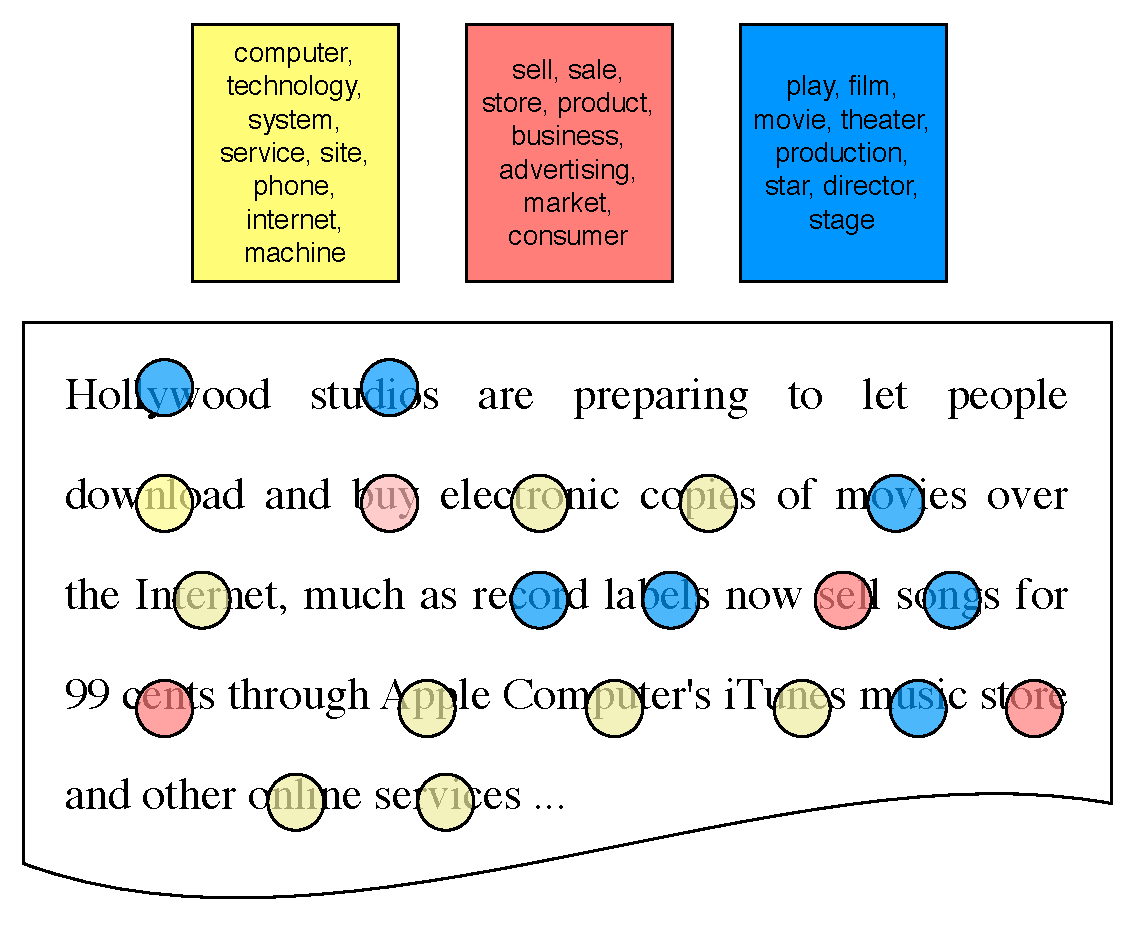
\includegraphics[width=.8\linewidth]{topic_models/inference_3}}
\only<2> {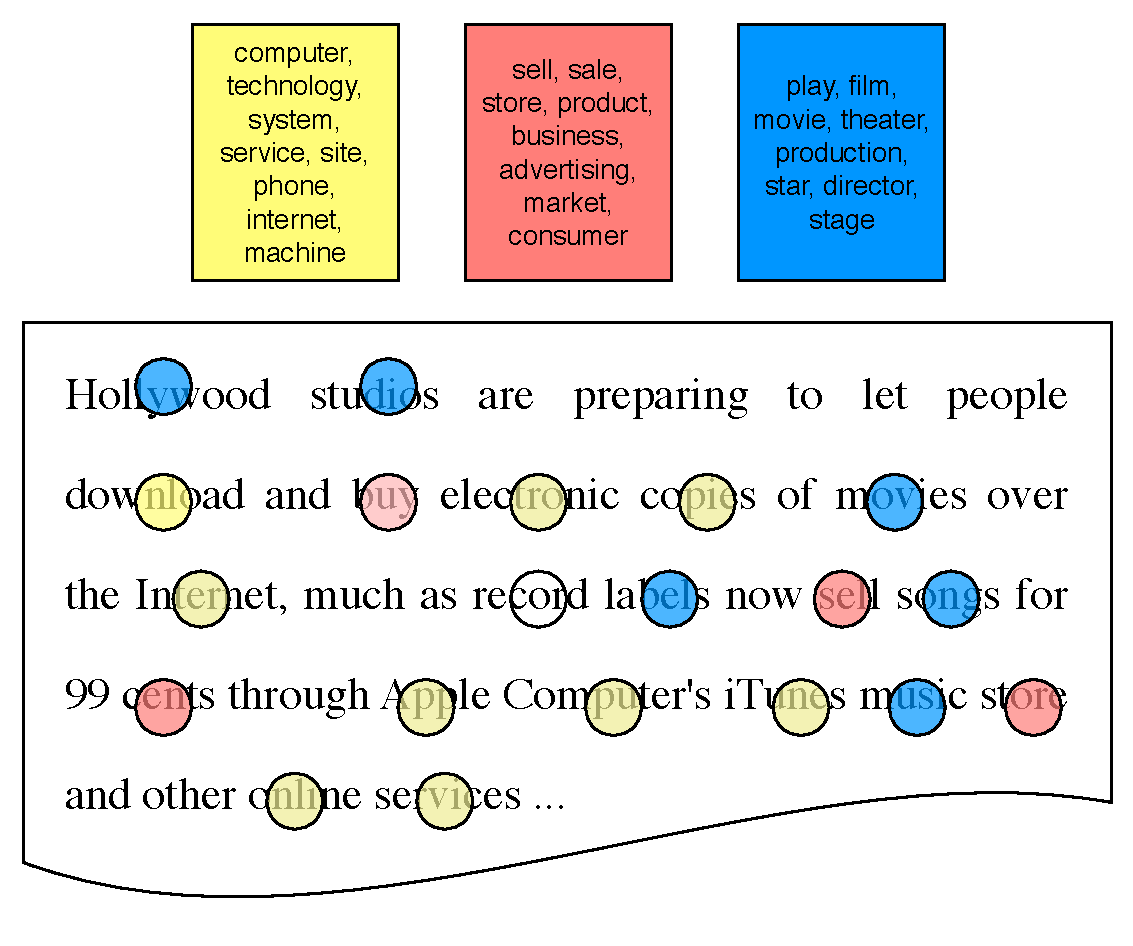
\includegraphics[width=.8\linewidth]{topic_models/inference_4}}
\only<3> {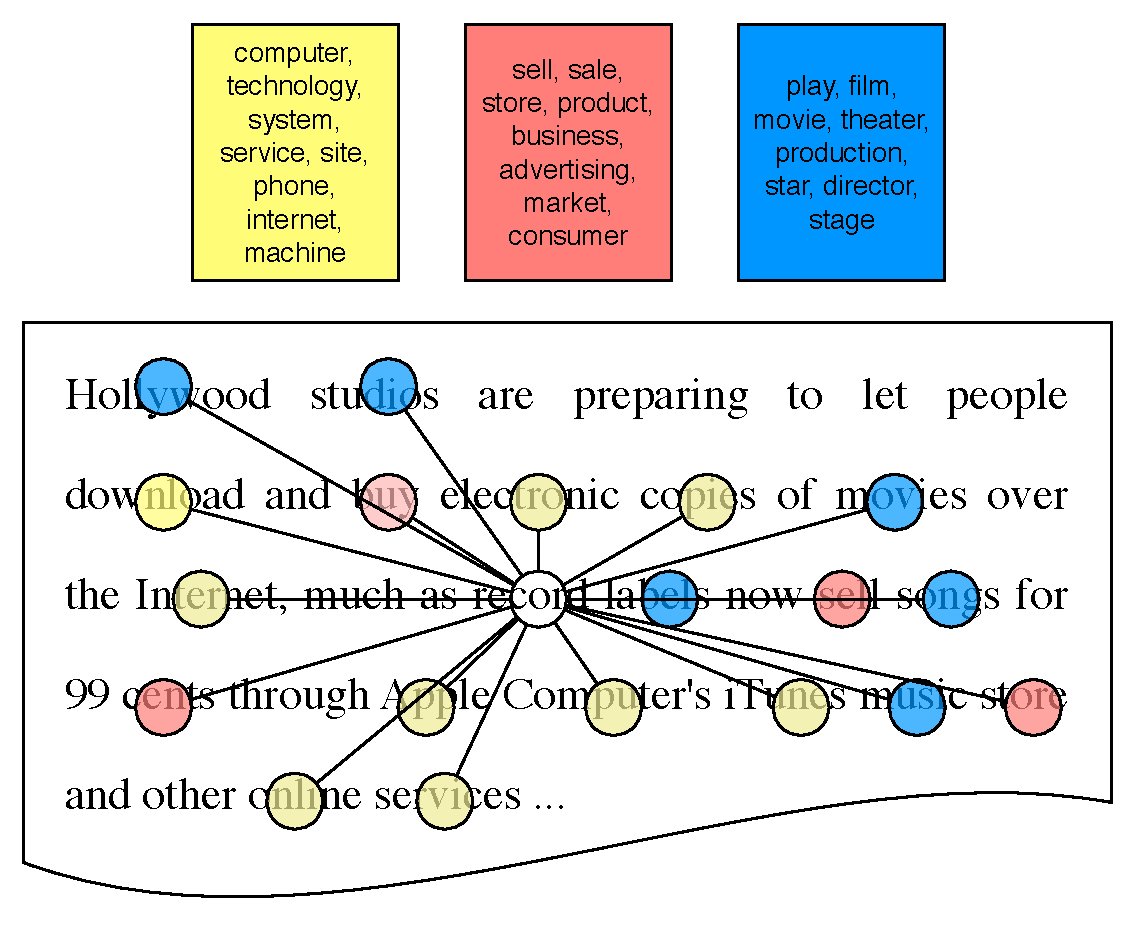
\includegraphics[width=.8\linewidth]{topic_models/inference_5}}
\only<4> {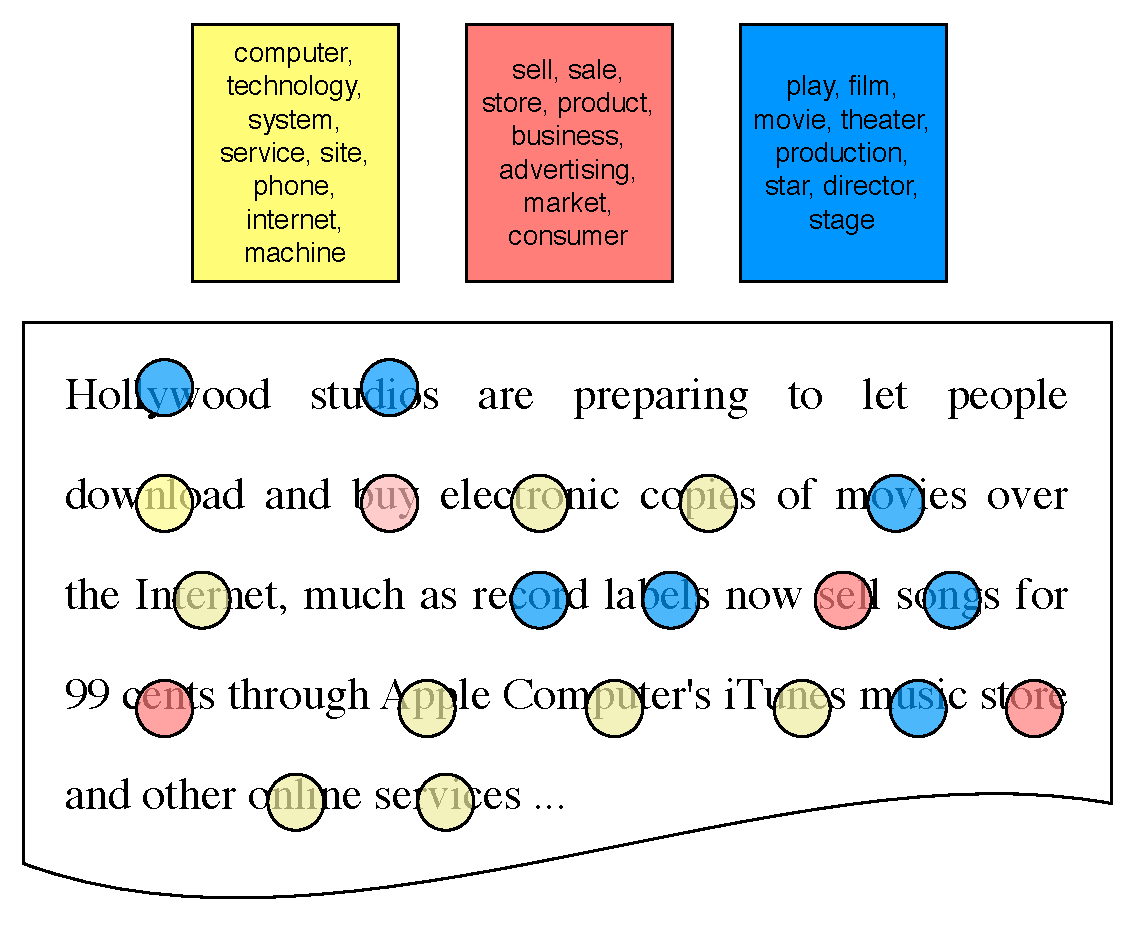
\includegraphics[width=.8\linewidth]{topic_models/inference_3}}
\only<5> {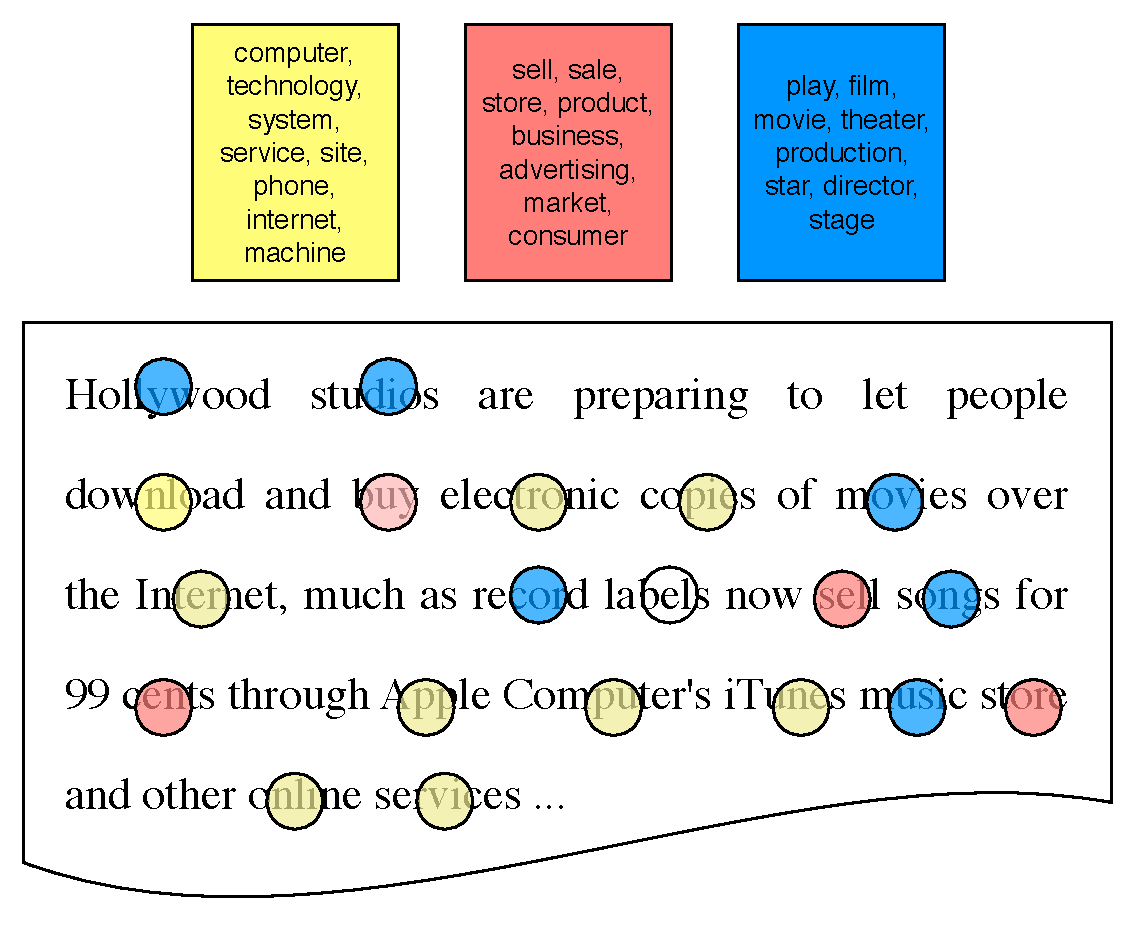
\includegraphics[width=.8\linewidth]{topic_models/inference_6}}
\only<6> {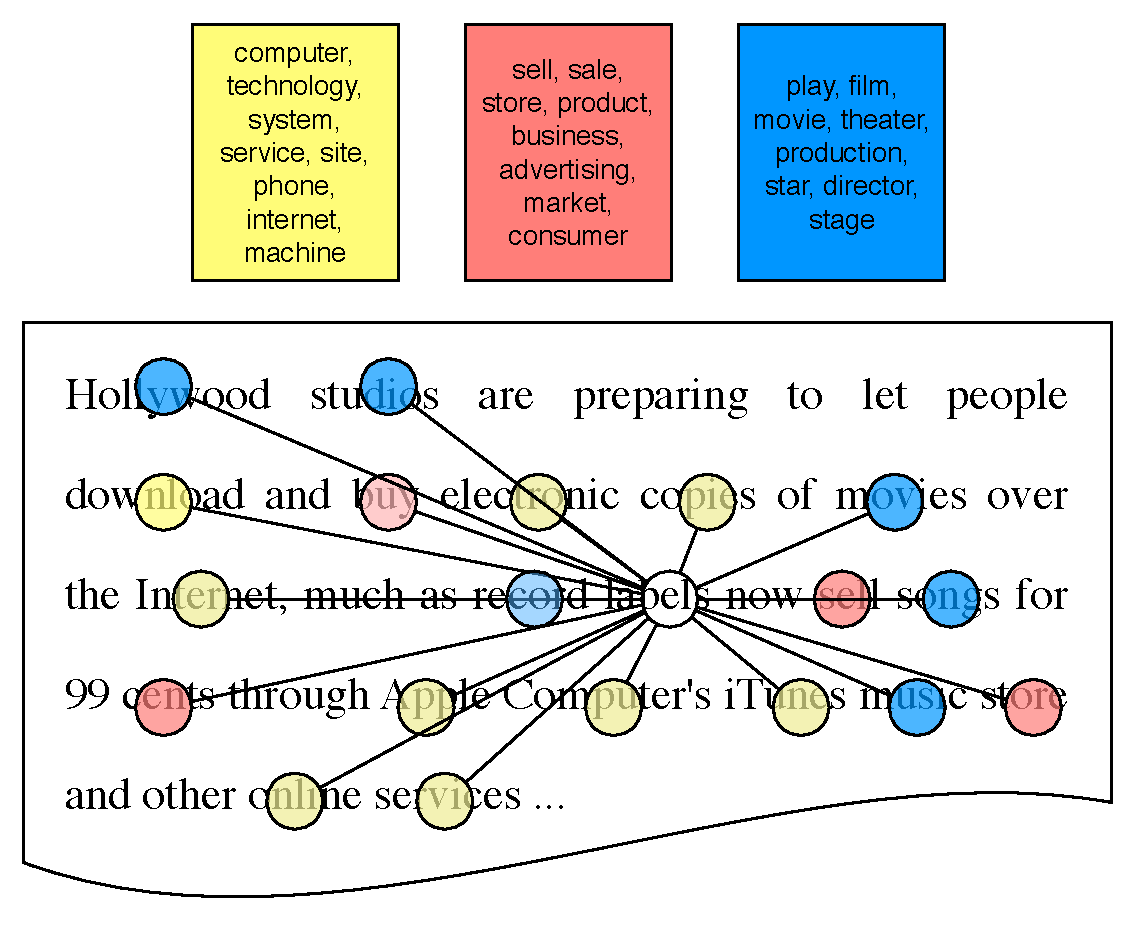
\includegraphics[width=.8\linewidth]{topic_models/inference_7}}
\only<7> {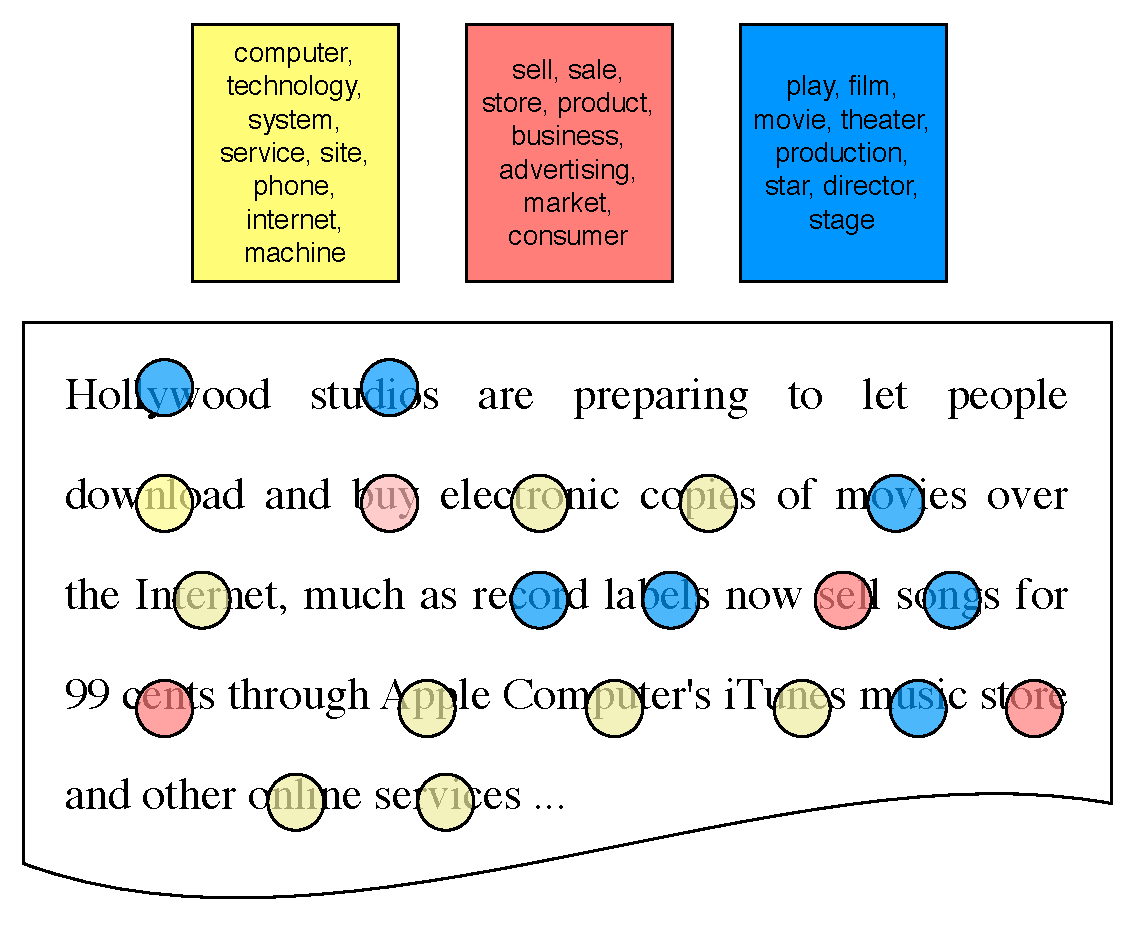
\includegraphics[width=.8\linewidth]{topic_models/inference_3}}
	\end{center}
}




\begin{frame}
\frametitle{Gibbs Sampling}
\begin{itemize}
\item For LDA, we will sample the topic assignments
\item Thus, we want:
\begin{equation*}
p(z_{d,n} = k | {\bm z}_{-d,n}, {\bm w}, \alpha, \lambda) = \frac{ p(z_{d,n} = k, {\bm z}_{-d,n} | {\bm w}, \alpha, \lambda)} { p({\bm z}_{-d,n} | {\bm w},\alpha, \lambda)}
\end{equation*}
\pause
\item The topics and per-document topic proportions are integrated out / marginalized
\item Let $n_{d,i}$ be the number of words taking topic $i$ in document $d$.  Let $v_{k,w}$ be the number of times word $w$ is used in topic $k$.
\end{itemize}


\begin{equation*}
= \frac{ \int_{\theta_d} \left( \prod_{i \not = k} \theta_d^{\alpha_i + n_{d,i} - 1} \right)\theta_d^{\alpha_k + n_{d,k} } d\theta_d \int_{\beta_{k}}    \left( \prod_{i \not = w_{d,n}} \beta_{k,i} ^{ \lambda_i + v_{k,i} - 1} \right) \beta_{k, w_{d,n}}^{\lambda_i + v_{k,w_{d,n}}} d\beta_k } { \int_{\theta_d} \left( \prod_{i} \theta_d^{\alpha_i + n_{d,i} - 1} \right) d\theta_d \int_{\beta_{k}}    \left( \prod_{i} \beta_{k,i} ^{ \lambda_i + v_{k,i} - 1} \right) d\beta_k }
\end{equation*}
\end{frame}





\begin{frame}
\frametitle{Gibbs Sampling}
\begin{itemize}
\item Integral is normalizer of Dirichlet distribution
\begin{equation*}
\int_{\beta_{k}}    \left( \prod_{i} \beta_{k,i} ^{ \lambda_i + v_{k,i} - 1} \right) d\beta_k = \dirfunc{i}{V}{\beta_i + v_{k,i}}
\end{equation*}
\pause
\item So we can simplify
\end{itemize}
\begin{footnotesize}
\begin{align*}
& \frac{ \int_{\theta_d} \left( \prod_{i \not = k} \theta_d^{\alpha_i + n_{d,i}
      - 1} \right)\theta_d^{\alpha_k + n_{d,k} } d\theta_d \int_{\beta_{k}}
  \left( \prod_{i \not = w_{d,n}} \beta_{k,i} ^{ \lambda_i + v_{k,i} - 1}
  \right) \beta_{k, w_{d,n}}^{\lambda_i + v_{k,w_{d,n}} d\beta_k } { \int_{\theta_d}
  \left( \prod_{i} \theta_d^{\alpha_i + n_{d,i} - 1} \right) d\theta_d
  \int_{\beta_{k}}    \left( \prod_{i} \beta_{k,i} ^{ \lambda_i + v_{k,i} - 1}
  \right) d\beta_k } = \\
& \frac{
  \dirnum{i \not = k}{K}{\alpha_k + n_{d,k} + 1}{ \G{\sum_{i}^{K} \alpha_i +
      n_{d,i} + 1} } \G{\alpha_k + n_{d,k}}  }
{ \dirfunc{i}{K}{\alpha_i + n_{d,i}} }
% -----------------------------------
\frac{
 \dirnum{i \not = w_{d,n}}{V}{\lambda_{w_{d,n}} + v_{k,w_{d,n}} + 1}{ \G{\sum_{i}^{V} \lambda_i + v_{k,i} + 1} } \G{\lambda_k + v_{k,w_{d,n}}}
}{ \dirfunc{i}{V}{\lambda_i + v_{k,i}} } \\
% -----------------------------------
\end{align*}
\end{footnotesize}
\end{frame}


\begin{frame}

\begin{block}{Gamma Function Identity}
	\begin{equation}
		z = \frac{\Gamma(z + 1)}{\Gamma(z)}
	\end{equation}
\end{block}

\begin{footnotesize}
\begin{align*}
& \frac{
  \dirnum{i \not = k}{K}{\alpha_k + n_{d,k} + 1}{ \G{\sum_{i}^{K} \alpha_i +
      n_{d,i} + 1} } \G{\alpha_k + n_{d,k}}  }
{ \dirfunc{i}{K}{\alpha_i + n_{d,i}} }
% -----------------------------------
\frac{
 \dirnum{i \not = w_{d,n}}{V}{\lambda_{w_{d,n}} + v_{k,w_{d,n}} + 1}{ \G{\sum_{i}^{V} \lambda_i + v_{k,i} + 1} } \G{\lambda_k + v_{k,w_{d,n}}}
}{ \dirfunc{i}{V}{\lambda_i + v_{k,i}} } \\
% -----------------------------------
& = \frac{n_{d, k} + \alpha_k}{ \sum_{i}^{K} { n_{d,i} + \alpha_i}} \frac{v_{k, w_{d,n}} + \lambda_{w_{d,n}}}{ \sum_{i} { v_{k,i} + \lambda_{i} }}
\end{align*}
\end{footnotesize}

\end{frame}

\begin{frame}{Gibbs Sampling Equation}

\begin{equation}
\alert<5>{\frac{\alert<1>{n_{d, k}} +  \alert<3>{\alpha_k}}{ \sum_{i}^{K} { n_{d,i} +\alpha_i}}} \alert<6>{\frac{\alert<2>{v_{k, w_{d,n}}} + \alert<4>{\lambda_{w_{d,n}}}}{ \sum_{i} { v_{k,i} + \lambda_{i} }}}
\end{equation}

\begin{itemize}
  \item \alert<1>{Number of times document $d$ uses topic $k$}
  \item \alert<2>{Number of times topic $k$ uses word type $w_{d,n}$}
  \item \alert<3>{Dirichlet parameter for document to topic
      distribution}
  \item \alert<4>{Dirichlet parameter for topic to word distribution}
  \item \alert<5>{How much this document likes topic $k$}
  \item \alert<6>{How much this topic likes word $w_{d,n}$}
\end{itemize}

\end{frame}

\begin{frame}
  \frametitle{Sample Document}
    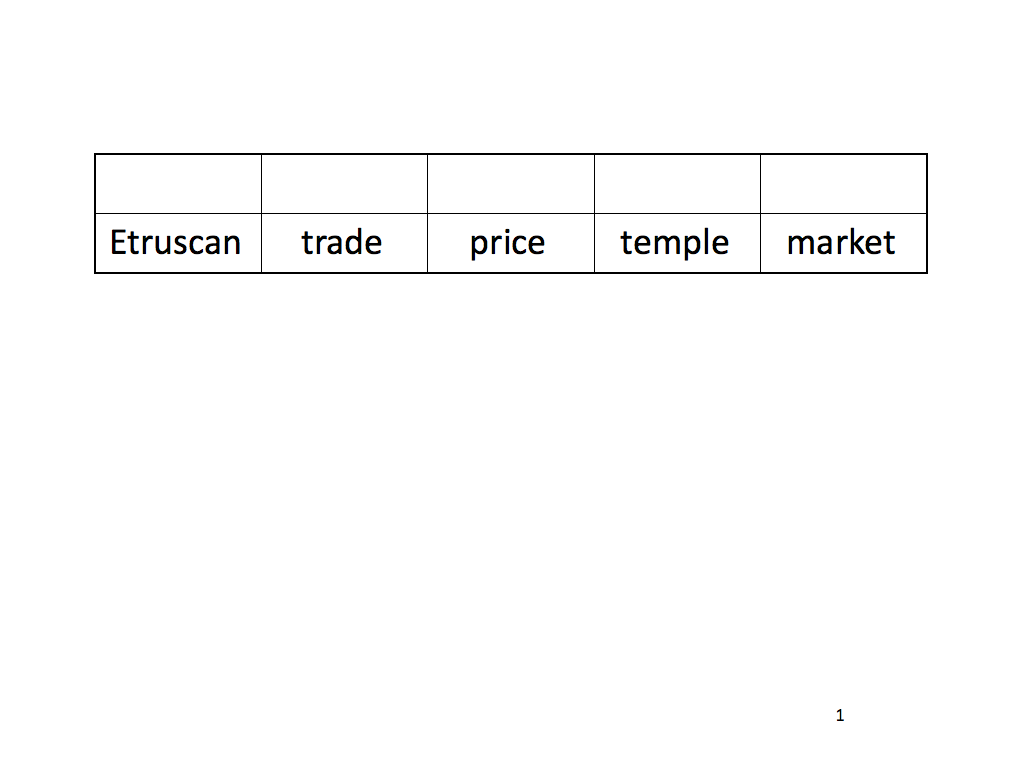
\includegraphics[width=\linewidth]{topic_models/mimno_001}
\end{frame}

\begin{frame}
  \frametitle{Sample Document}
    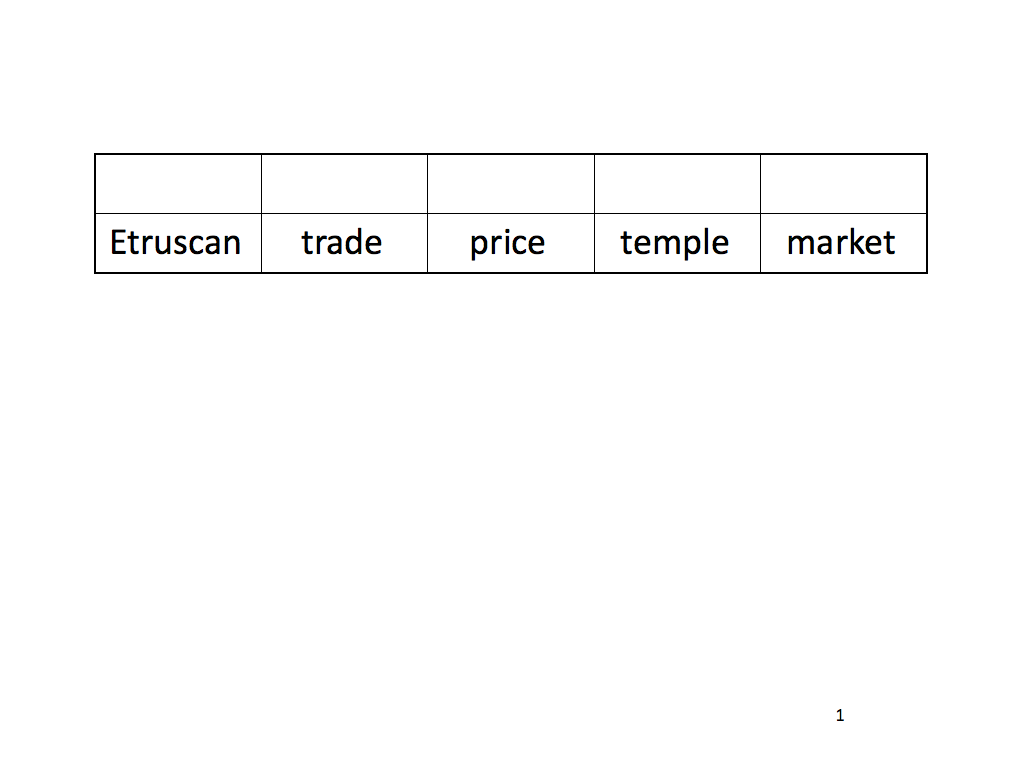
\includegraphics[width=\linewidth]{topic_models/mimno_001}
\end{frame}

\begin{frame}
  \frametitle{Randomly Assign Topics}
    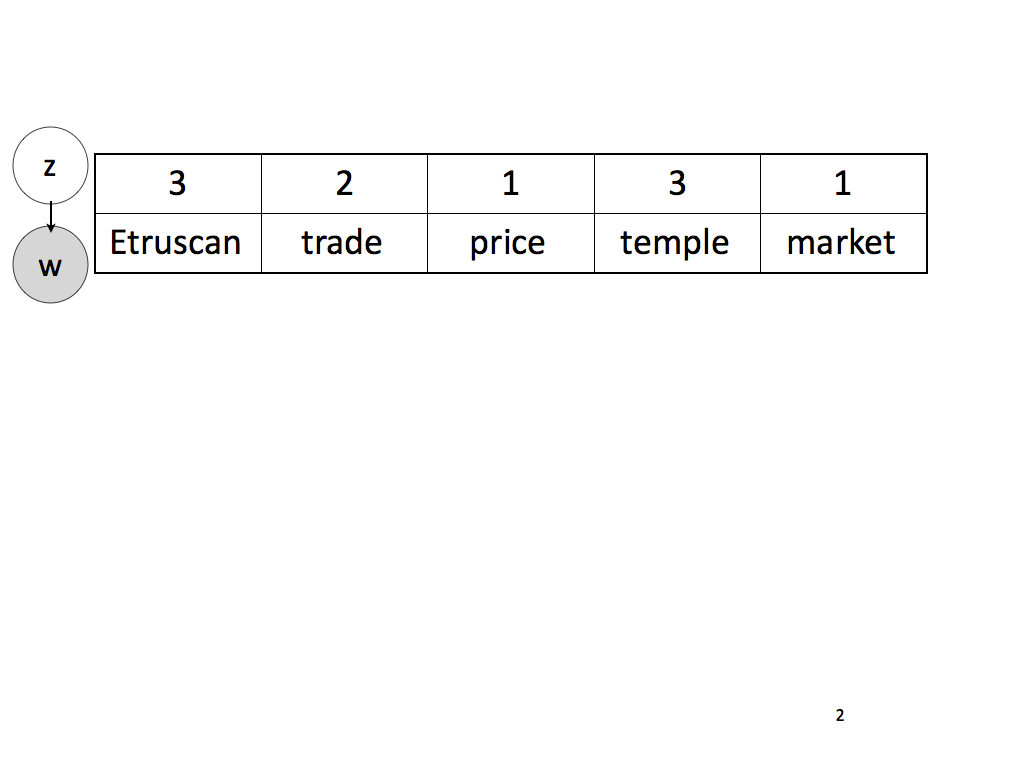
\includegraphics[width=\linewidth]{topic_models/mimno_002}
\end{frame}

\begin{frame}
  \frametitle{Randomly Assign Topics}
    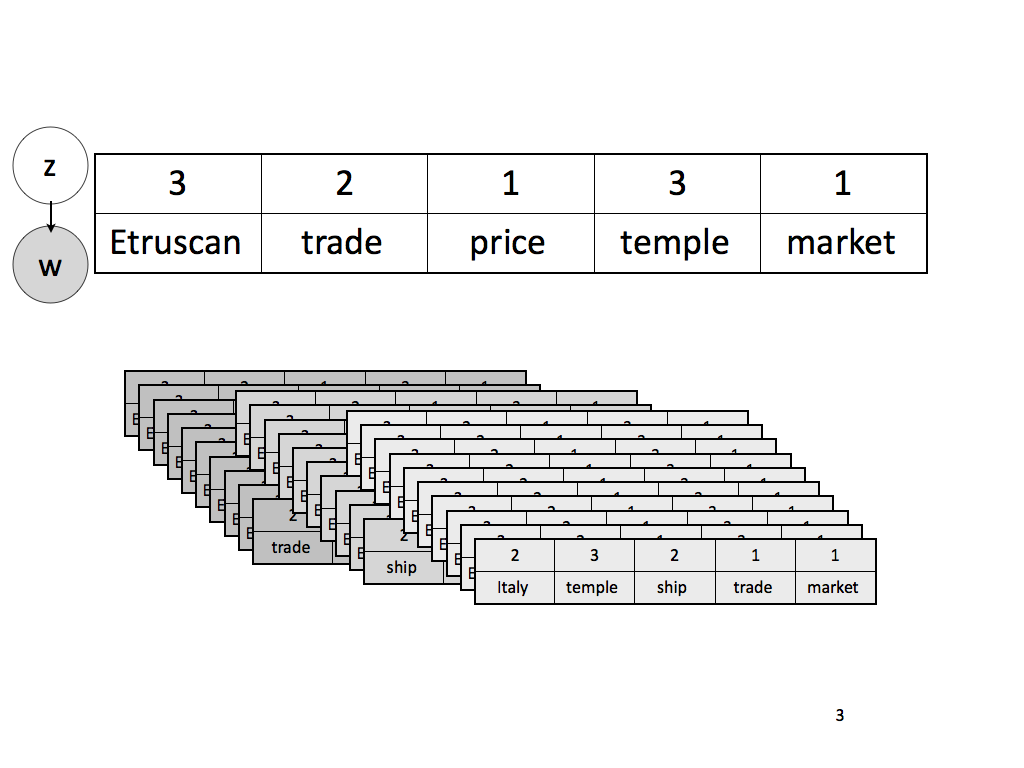
\includegraphics[width=\linewidth]{topic_models/mimno_003}
\end{frame}

\begin{frame}
  \frametitle{Total Topic Counts}
    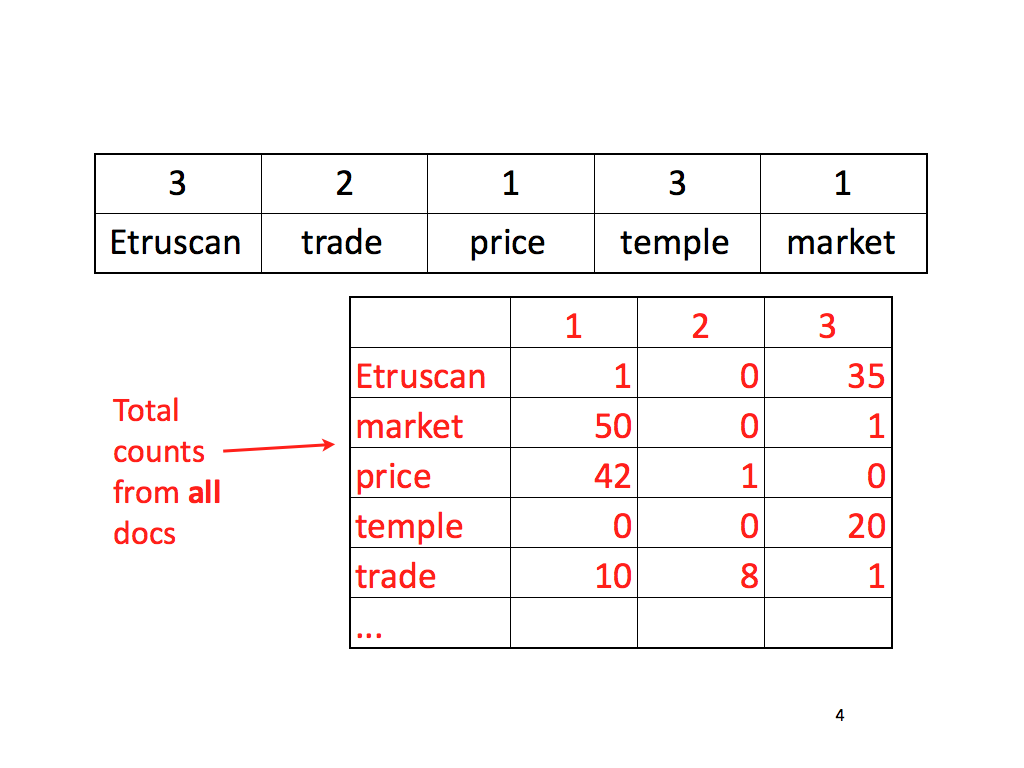
\includegraphics[width=\linewidth]{topic_models/mimno_004}

\pause

\vspace{-4cm}

\begin{block}{Sampling Equation}
	\begin{equation*}
          \frac{n_{d, k} + \alpha_k}{ \sum_{i}^{K} { n_{d,i} + \alpha_i}} \frac{\alert<3>{v_{k, w_{d,n}}} + \lambda_{w_{d,n}}}{ \sum_{i} { \alert<3>{v_{k,i}} + \lambda_{i} }}
	\end{equation*}
\end{block}

\end{frame}


\begin{frame}
  \frametitle{We want to sample this word \dots}
    \only<1>{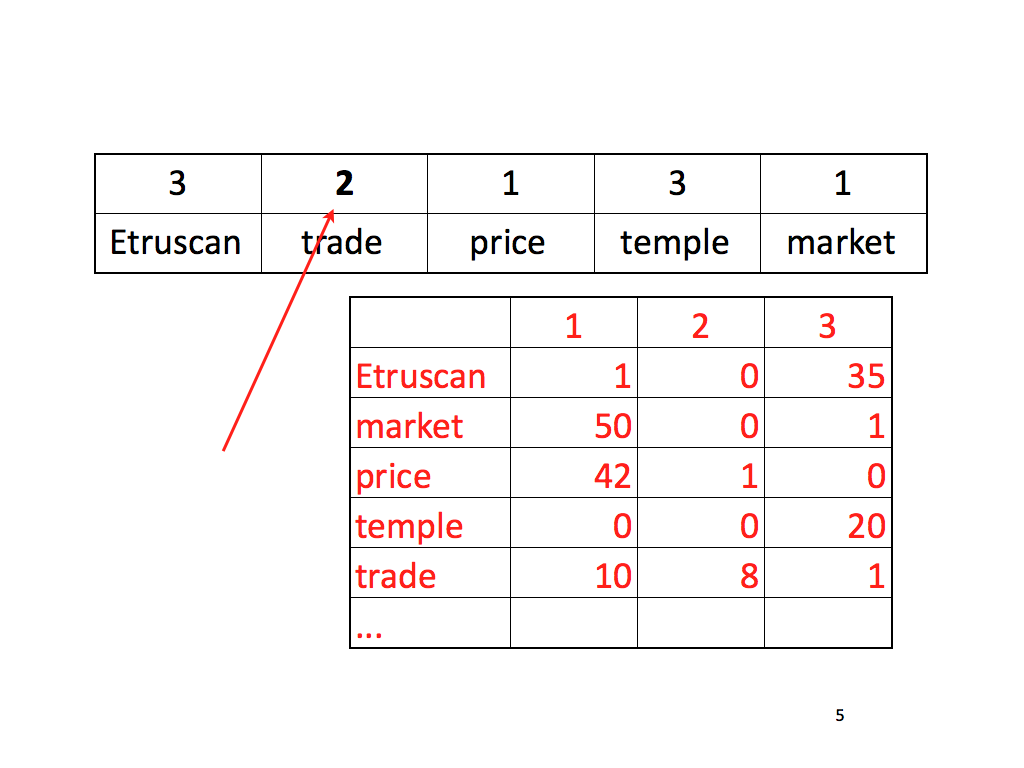
\includegraphics[width=\linewidth]{topic_models/mimno_005}}
    \only<2>{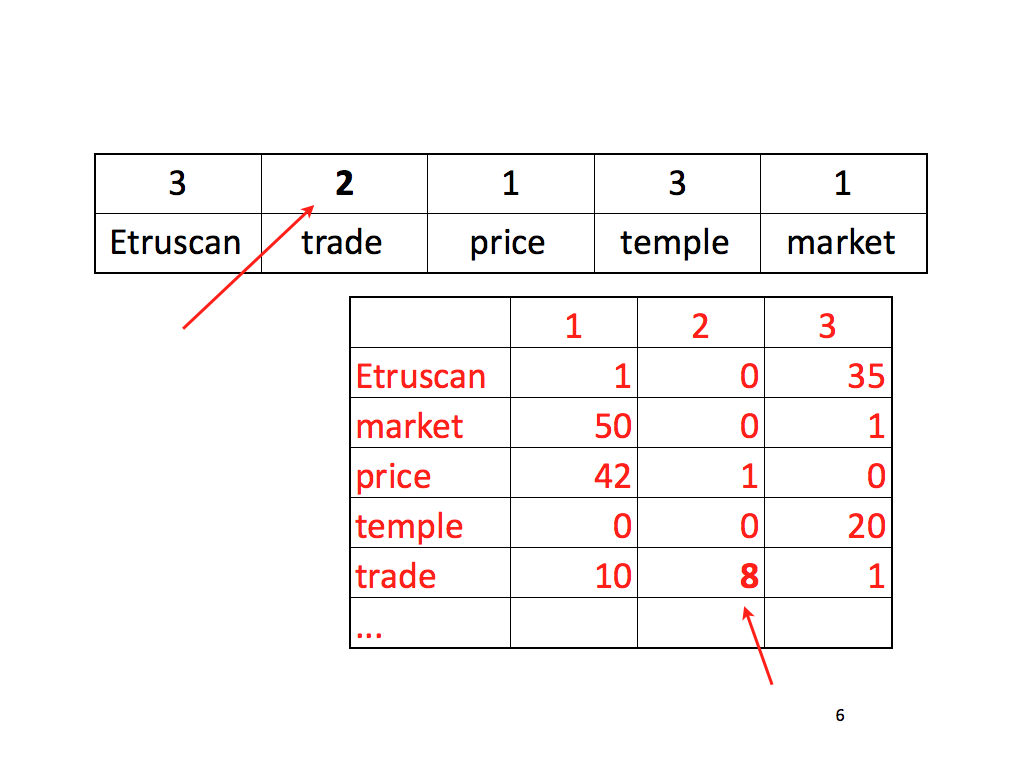
\includegraphics[width=\linewidth]{topic_models/mimno_006}}
\end{frame}

\begin{frame}
  \frametitle{Decrement its count}
    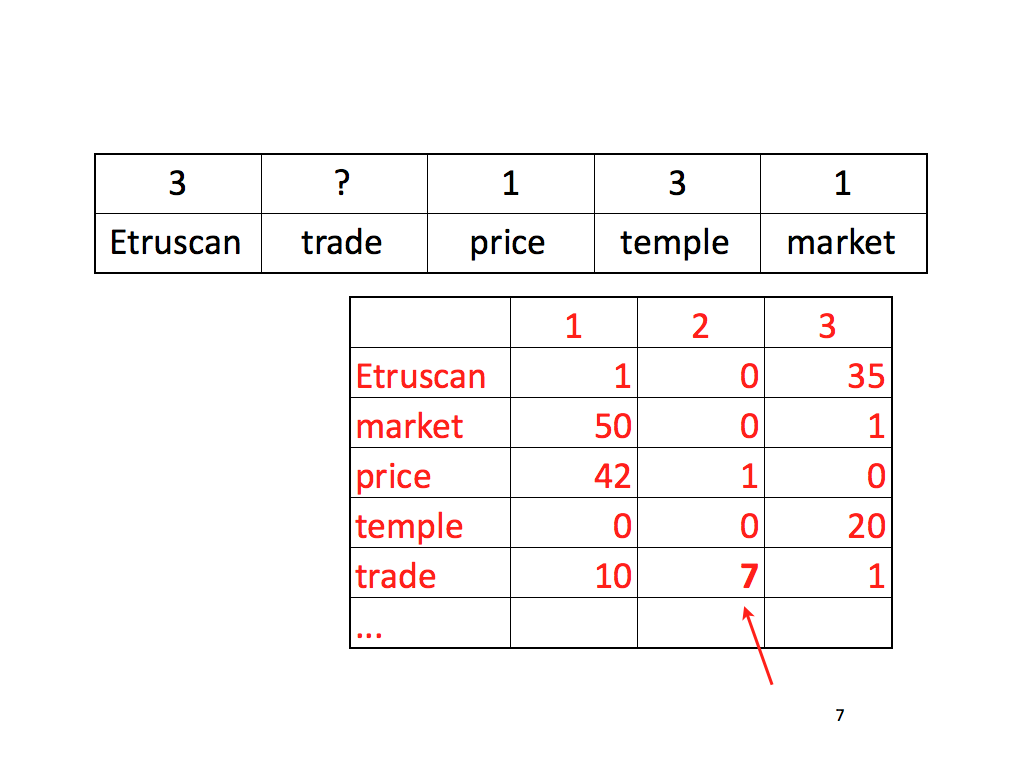
\includegraphics[width=\linewidth]{topic_models/mimno_007}
\end{frame}

\begin{frame}
  \frametitle{What is the conditional distribution for this topic?}
    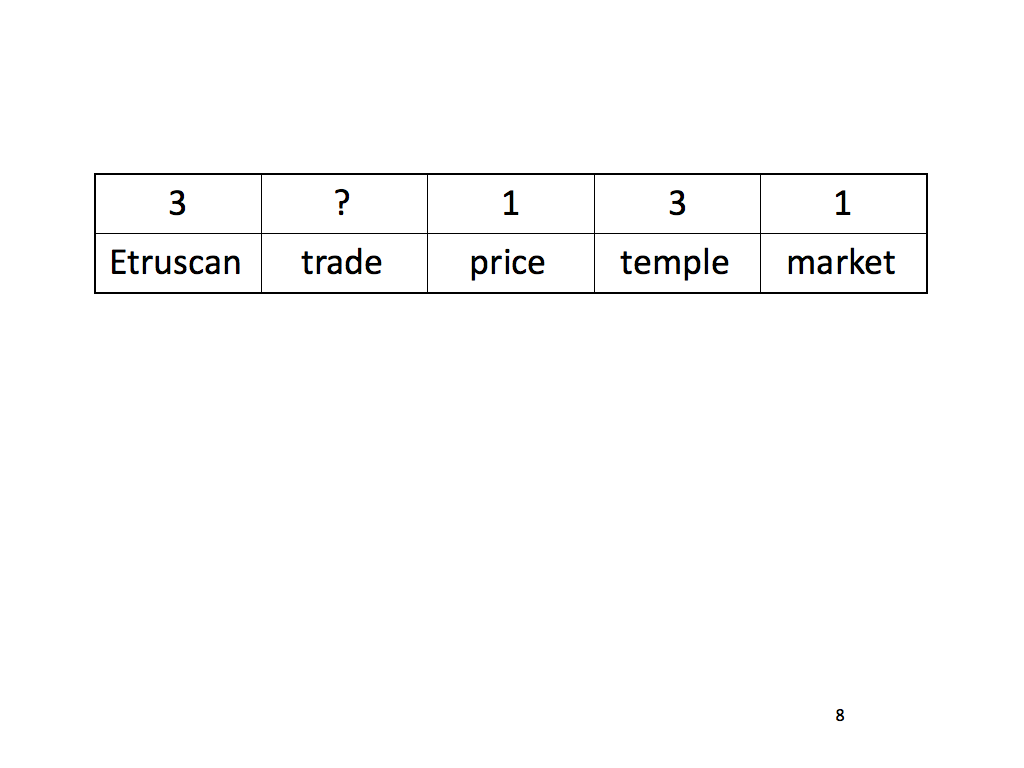
\includegraphics[width=\linewidth]{topic_models/mimno_008}
\end{frame}


\begin{frame}
  \frametitle{Part 1: How much does this document like each topic?}
    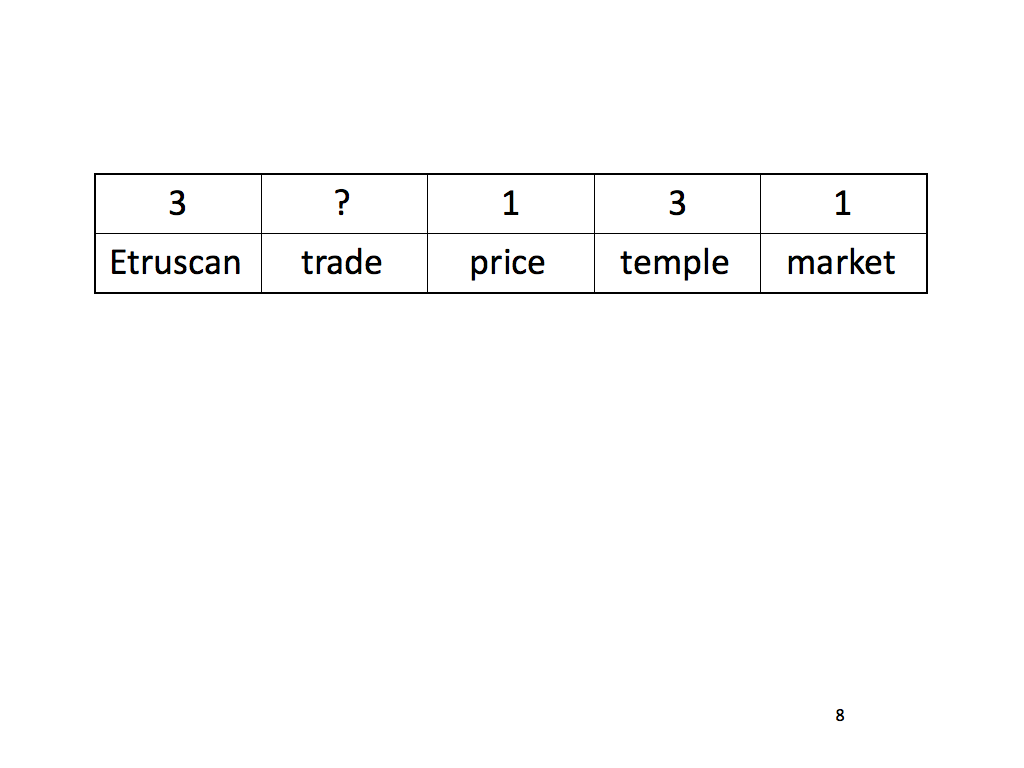
\includegraphics[width=\linewidth]{topic_models/mimno_008}
\end{frame}

\begin{frame}
  \frametitle{Part 1: How much does this document like each topic?}
    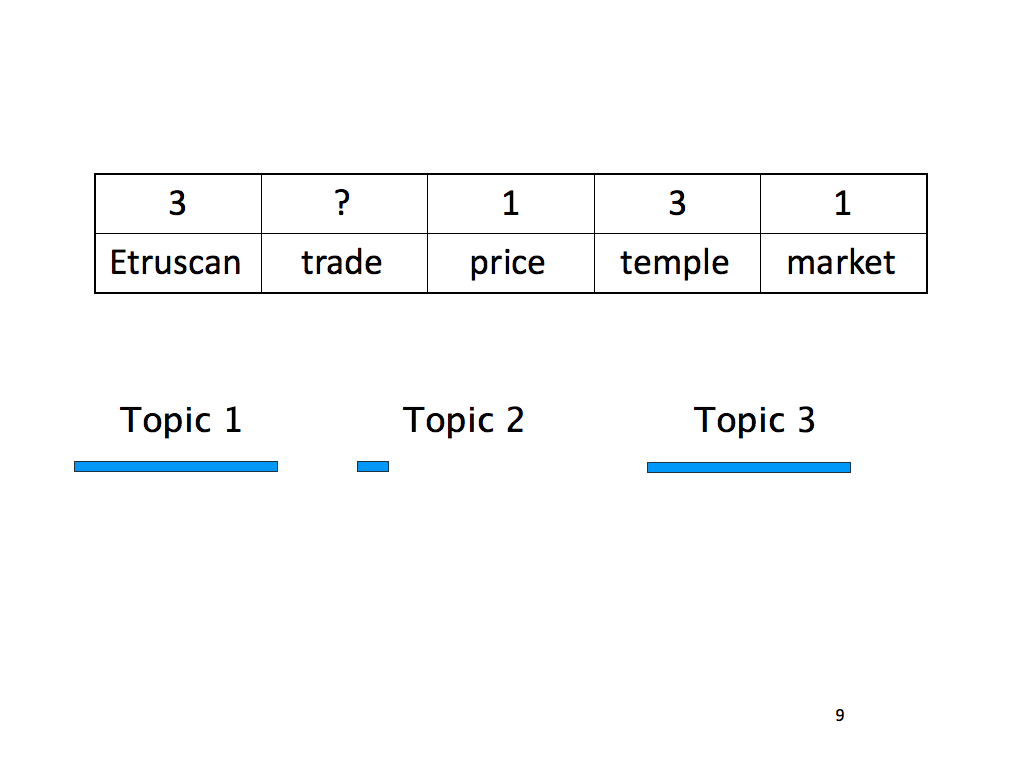
\includegraphics[width=\linewidth]{topic_models/mimno_009}

    \pause
    \vspace{-4cm}
    \begin{block}{Sampling Equation}
	\begin{equation*}
          \frac{\alert<3>{n_{d, k}} + \alpha_k}{ \sum_{i}^{K} { \alert<3>{n_{d,i}} + \alpha_i}} \frac{v_{k, w_{d,n}} + \lambda_{w_{d,n}}}{ \sum_{i} { v_{k,i} + \lambda_{i} }}
	\end{equation*}
     \end{block}


\end{frame}


\begin{frame}
  \frametitle{Part 2: How much does each topic like the word?}
    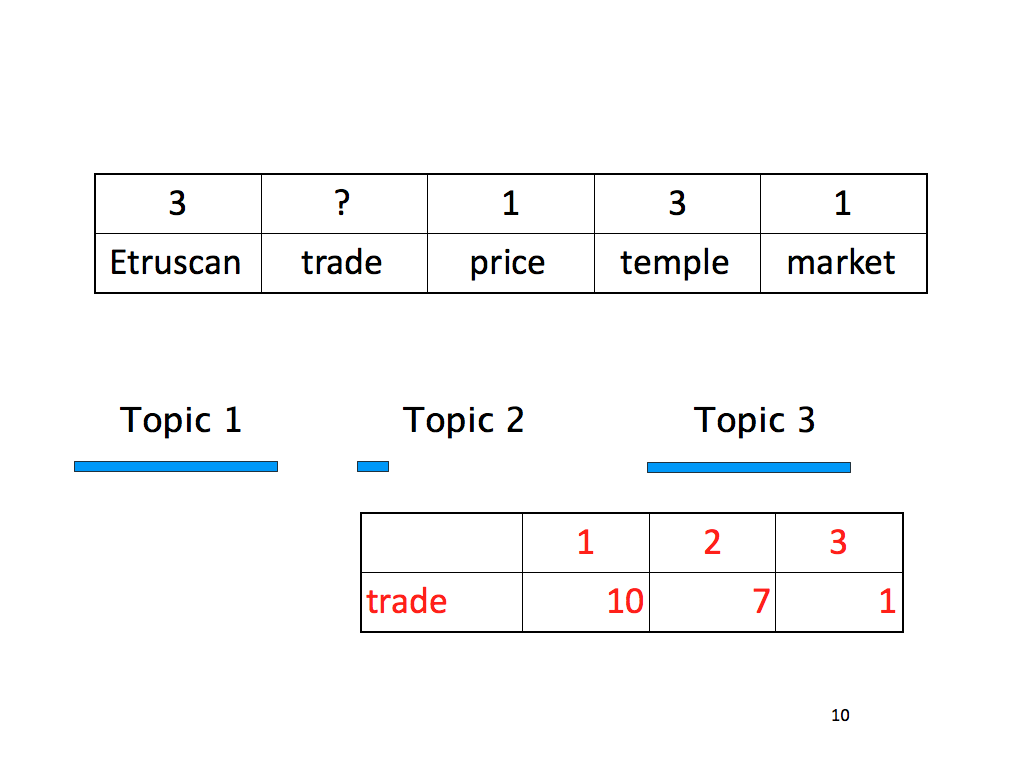
\includegraphics[width=\linewidth]{topic_models/mimno_010}

\pause

\vspace{-4cm}

\begin{block}{Sampling Equation}
	\begin{equation*}
          \frac{n_{d, k} + \alpha_k}{ \sum_{i}^{K} { n_{d,i} + \alpha_i}} \frac{\alert<3>{v_{k, w_{d,n}}} + \lambda_{w_{d,n}}}{ \sum_{i} { \alert<3>{v_{k,i}} + \lambda_{i} }}
	\end{equation*}
\end{block}

\end{frame}


\begin{frame}
  \frametitle{Geometric interpretation}
    \only<1>{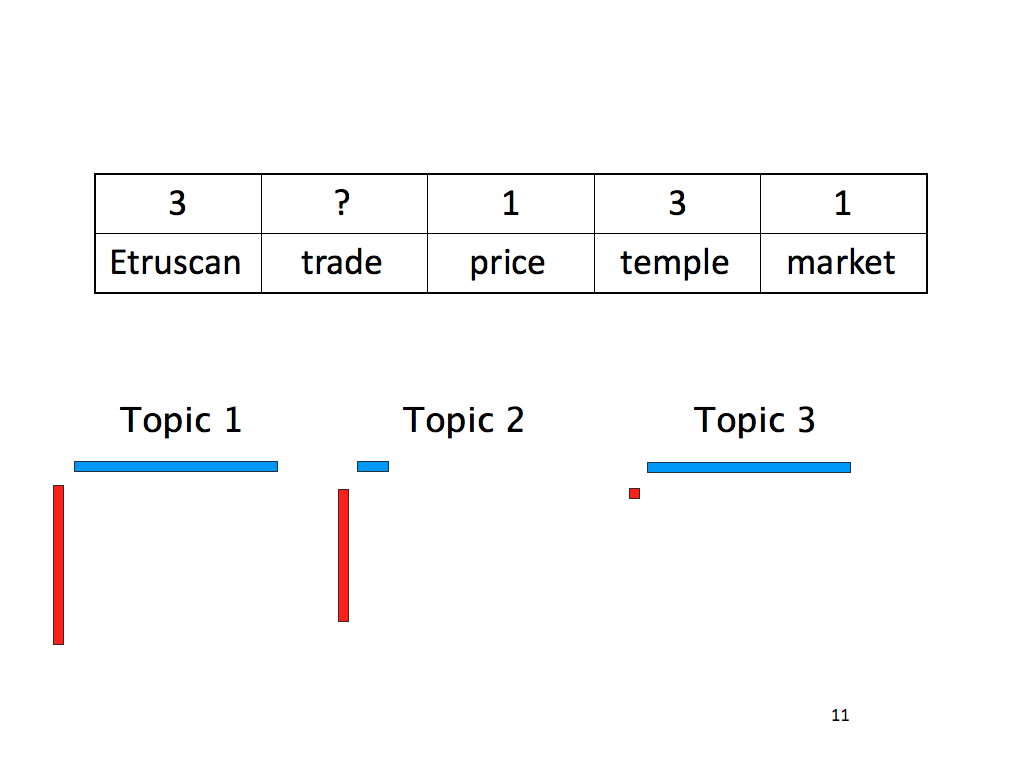
\includegraphics[width=\linewidth]{topic_models/mimno_011}}
    \only<2>{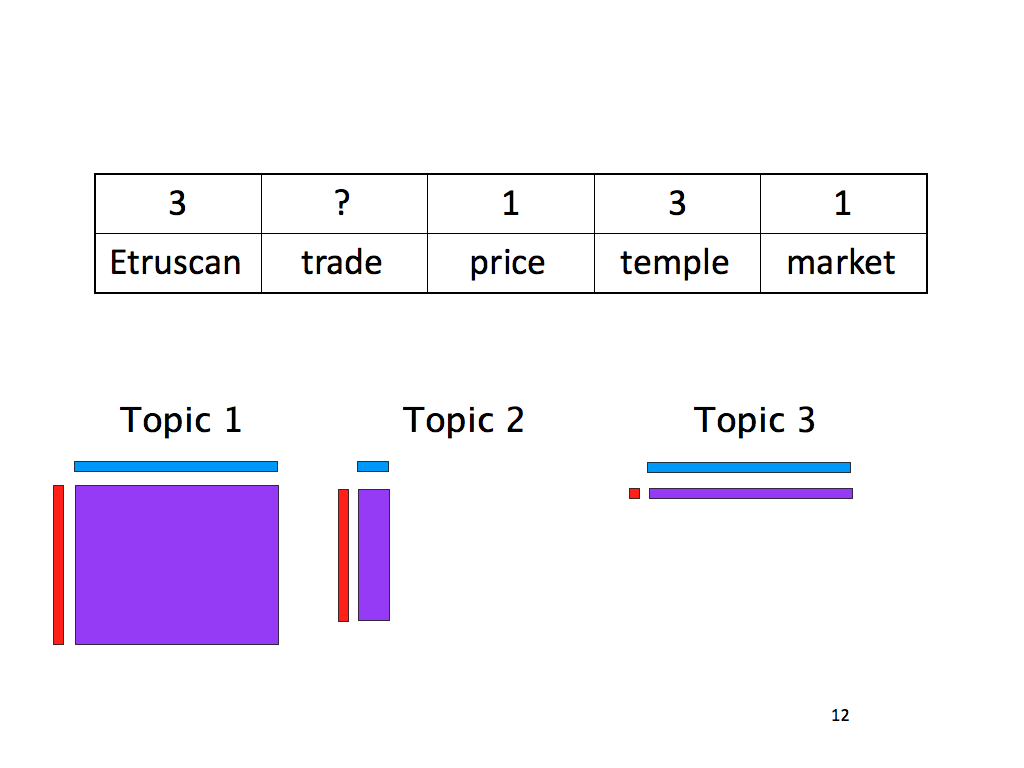
\includegraphics[width=\linewidth]{topic_models/mimno_012}}
    \only<3>{\includegraphics[width=\linewidth]{topic_models/mimno_013}}
\end{frame}

\begin{frame}
  \frametitle{Update counts}
    \only<1>{\includegraphics[width=\linewidth]{topic_models/mimno_014}}
    \only<2>{\includegraphics[width=\linewidth]{topic_models/mimno_015}}
    \only<3>{\includegraphics[width=\linewidth]{topic_models/mimno_016}}
\end{frame}


\begin{frame}
  \frametitle{Details: how to sample from a distribution}

\begin{center}
  \includegraphics[width=.8\linewidth]{topic_models/sampling_from_distribution}
\end{center}
\end{frame}

\begin{frame}

\begin{block}{Algorithm}
\begin{enumerate}
\item For each iteration $i$:
\begin{enumerate}
\item For each document $d$ and word $n$ currently assigned to $z_{old}$:
\begin{enumerate}
\item Decrement $n_{d,z_{old}}$ and $v_{z_{old}, w_{d,n}}$
\item Sample $z_{new} = k$ with probability proportional to $\frac{n_{d, k} + \alpha_k}{ \sum_{i}^{K} { n_{d,i} + \alpha_i}} \frac{v_{k, w_{d,n}} + \lambda_{w_{d,n}}}{ \sum_{i} { v_{k,i} + \lambda_{i}}}$
\item Increment $n_{d,z_{new}}$ and $v_{z_{new}, w_{d,n}}$
\end{enumerate}
\end{enumerate}
\end{enumerate}
\end{block}

\end{frame}

\begin{frame}

\frametitle{Implementation}

\begin{block}{Algorithm}
\begin{enumerate}
\item For each iteration $i$:
\begin{enumerate}
\item For each document $d$ and word $n$ currently assigned to $z_{old}$:
\begin{enumerate}
\item Decrement $n_{d,z_{old}}$ and $v_{z_{old}, w_{d,n}}$
\item Sample $z_{new} = k$ with probability proportional to $\frac{n_{d, k} + \alpha_k}{ \sum_{i}^{K} { n_{d,i} + \alpha_i}} \frac{v_{k, w_{d,n}} + \lambda_{w_{d,n}}}{ \sum_{i} { v_{k,i} + \lambda_{i}}}$
\item Increment $n_{d,z_{new}}$ and $v_{z_{new}, w_{d,n}}$
\end{enumerate}
\end{enumerate}
\end{enumerate}
\end{block}

\end{frame}


\begin{frame}
\frametitle{Desiderata}
\begin{itemize}
\item Hyperparameters: Sample them too (slice sampling)
\item Initialization: Random
\item Sampling: Until likelihood converges
\item Lag / burn-in: Difference of opinion on this
\item Number of chains: Should do more than one
\end{itemize}
\end{frame}

\begin{frame}
	\frametitle{Available implementations}

	\begin{itemize}
		\item Mallet (http://mallet.cs.umass.edu)
		\item LDAC (http://www.cs.princeton.edu/~blei/lda-c)
		\item Topicmod (http://code.google.com/p/topicmod)
	\end{itemize}
\end{frame}

\begin{frame}
\bibliographystyle{plain}
\tiny
\bibliography{bib/journal-full,bib/jbg}
\end{frame}

\end{document}
